% !TeX root = ../analysisnote.tex

\section{Analysis method}
In this section, event plane reconstruction would be described firstly.
Second part is identification for measured particles, including identified particles($\pi^+$ and $\pi^-$), 
and weak decay particles($K_0^S$ and $\Lambda$). Last one is efficiency correction, 
including TPC tracking efficiency, TOF matching efficiency and particle reconstruction efficiency.


\subsection{Event plane reconstruction}
Event plane method is one of common method in the anisotropic flow analysis, which could be used to estimate
the reaction plane in the Heavy Ion Collision.\cite{PhysRevC.83.044913} In this analysis, we used STAR detector 
Event Plane Detector(EPD), incorporating with Time Projection Chamber to reconstructe Event Plane(EP), 
where EPD is an upgrade detector in the STAR Beam Energy Scan phase II.\cite{ADAMS2020163970} There are 12 supersectors
on EPD. And 31 tiles on each supersector are connected via optical fiber bundles.
The tile performance would be affected by its own quality and the signal intensity it received.
So the correction for each tile is necessary, which would be introduced as follow.

Recentering and shifting method are two methods which we applied to correct the raw event plane
distribution. EPD is divided to four ring groups to facilitate EP reconstruction. There are 16 rings/rows
on EPD. It is divided equally to four groups, each group have four rings. Fig.~\ref{fig:EPDgroup} show
\begin{figure}[hbt!]
\centering
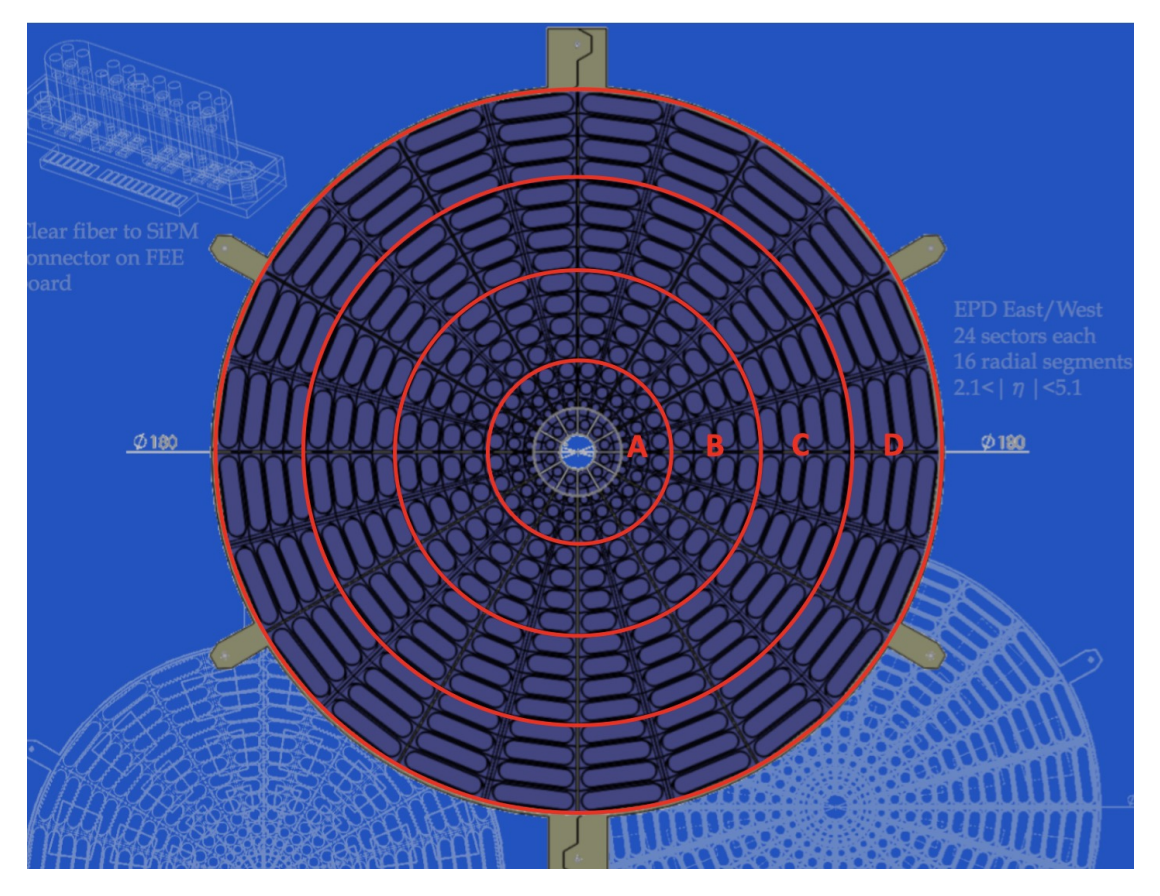
\includegraphics[width=0.45\linewidth]{figures/chapter02/EPDgroup.png}
\caption{The sketch of EPD groups.}
\label{fig:EPDgroup}
\end{figure}
groups at EPD, named as A, B, C and D. The best EP should be the one in the forward eta range, where directed flow
signal is greater than the one in middle eta range. \href{https://drupal.star.bnl.gov/STAR/system/files/FXT3gev_note_v4.pdf}{Analysis note} of one STAR published paper have approved it. 
We followed and chose EPD group A and B as target event plane in our analysis.
In this way, we can get the largest resolution applied to our analysis according to equation~\ref{eq:res_simp}
\begin{equation}
    R_n \propto v_n \sqrt{M}
\label{eq:res_simp}
\end{equation}

\subsubsection{Recentering correction}
The recentering calibration is applied to the flow vector($\vec{Q}$), which could be decomposed into 
two components, as shown by equation~\ref{eq:Qvector}, where $w_i$ is EPD tile weight, using the
calibrated value nMip(also known as ADC) based on the particle energy loss on each EPD tile, as shown by equation~\ref{eq:tile_weight}
\begin{equation}
    \overrightarrow{\mathrm{Q}}=\left(\begin{array}{l}
    Q_y \\
    Q_x
    \end{array}\right)=\left(\begin{array}{c}
    \sum_i w_i \sin (\phi_i) \\
    \sum_i w_i \cos (\phi_i)
    \end{array}\right)
\label{eq:Qvector}
\end{equation}

\begin{equation}
    w(\text { tile })= \begin{cases}0 & \text { if } n M I P<\operatorname{threshold}(0.3) \\ \text { MAX } & \text { if nMIP }>\operatorname{MAX}(2) \\ n M I P & \text { otherwise }\end{cases}
\label{eq:tile_weight}
\end{equation}
And the first order event plane angle could be obtained by equation~\ref{eq:EPangle}, where $\phi_i$ is emitted particle angle 
with respect to the laboratory system, sums goes over all hits from one event.
\begin{equation}
    \Psi_1=\tan ^{-1} \frac{\sum_i w_i \sin \left(\phi_i\right)}{\sum_i w_i \cos \left(\phi_i\right)}
\label{eq:EPangle}
\end{equation}

The recentering method is applied to the flow vertex $\vec{Q}$, so it's event by event calibration,
Which is expressed by equation~\ref{eq:recenter_method}. The angle brackets denote averaging over all events
in the same centrality and run ID.
\begin{equation}
    \vec{Q}_{r c}=\left(\begin{array}{l}
    \vec{Q}_y-\left\langle\vec{Q}_y\right\rangle \\
    \vec{Q}_x-\left\langle\vec{Q}_x\right\rangle
    \end{array}\right)
\label{eq:recenter_method}
\end{equation}

\subsubsection{Shifting correction}
The shifting calibration is a mathematical method to correct the EP distribution after recentering calibration,
which is based on Fourier transformation. In this analysis, a 20th order equation~\ref{eq:shift_method} was implemented to the event plane distribution
after recentering calibration.
\begin{equation}
\Psi_{1, \text { shift }}=\sum_i^N \frac{2}{i}\left[-\left\langle\sin \left(i \Psi_{1, r c}\right)\right\rangle \cos \left(i \Psi_{1, r c}\right)+\left\langle\cos \left(i \Psi_{1, r c}\right)\right\rangle \sin \left(i \Psi_{1, r c}\right)\right]
\label{eq:shift_method}
\end{equation}

The angle brackets in the equation denote averaging over all events in the same centrality and run ID.
And the final EP angle after recentering and shifting calibration could be obtained by equation~\ref{eq:psi_final}
\begin{equation}
\Psi_1=\Psi_{1, r c}+\Psi_{1, s h i f t}
\label{eq:psi_final}
\end{equation}

Fig.~\ref{fig:EP_distribution} show event plane distribution at 3, 3.2, 3.5 and 3.9 GeV based on all EPD rings,
where the black line show the raw distribution without any calibration, the blue line represents the EP after recentering calibration, 
and red line denote the event plane angle distribution after recentering and shifting calibration, which is "flat".
\begin{figure}[hbt!]
\centering
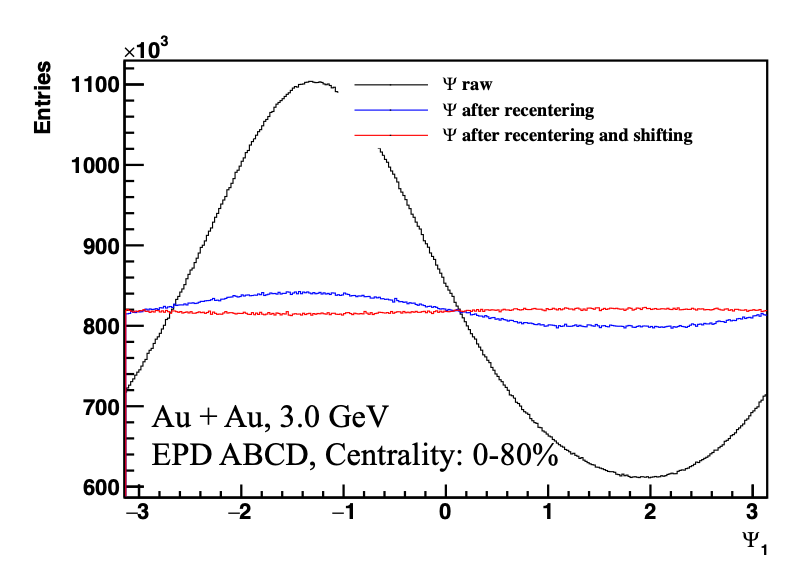
\includegraphics[width=0.45\linewidth]{figures/chapter02/EP_3GeV.png}
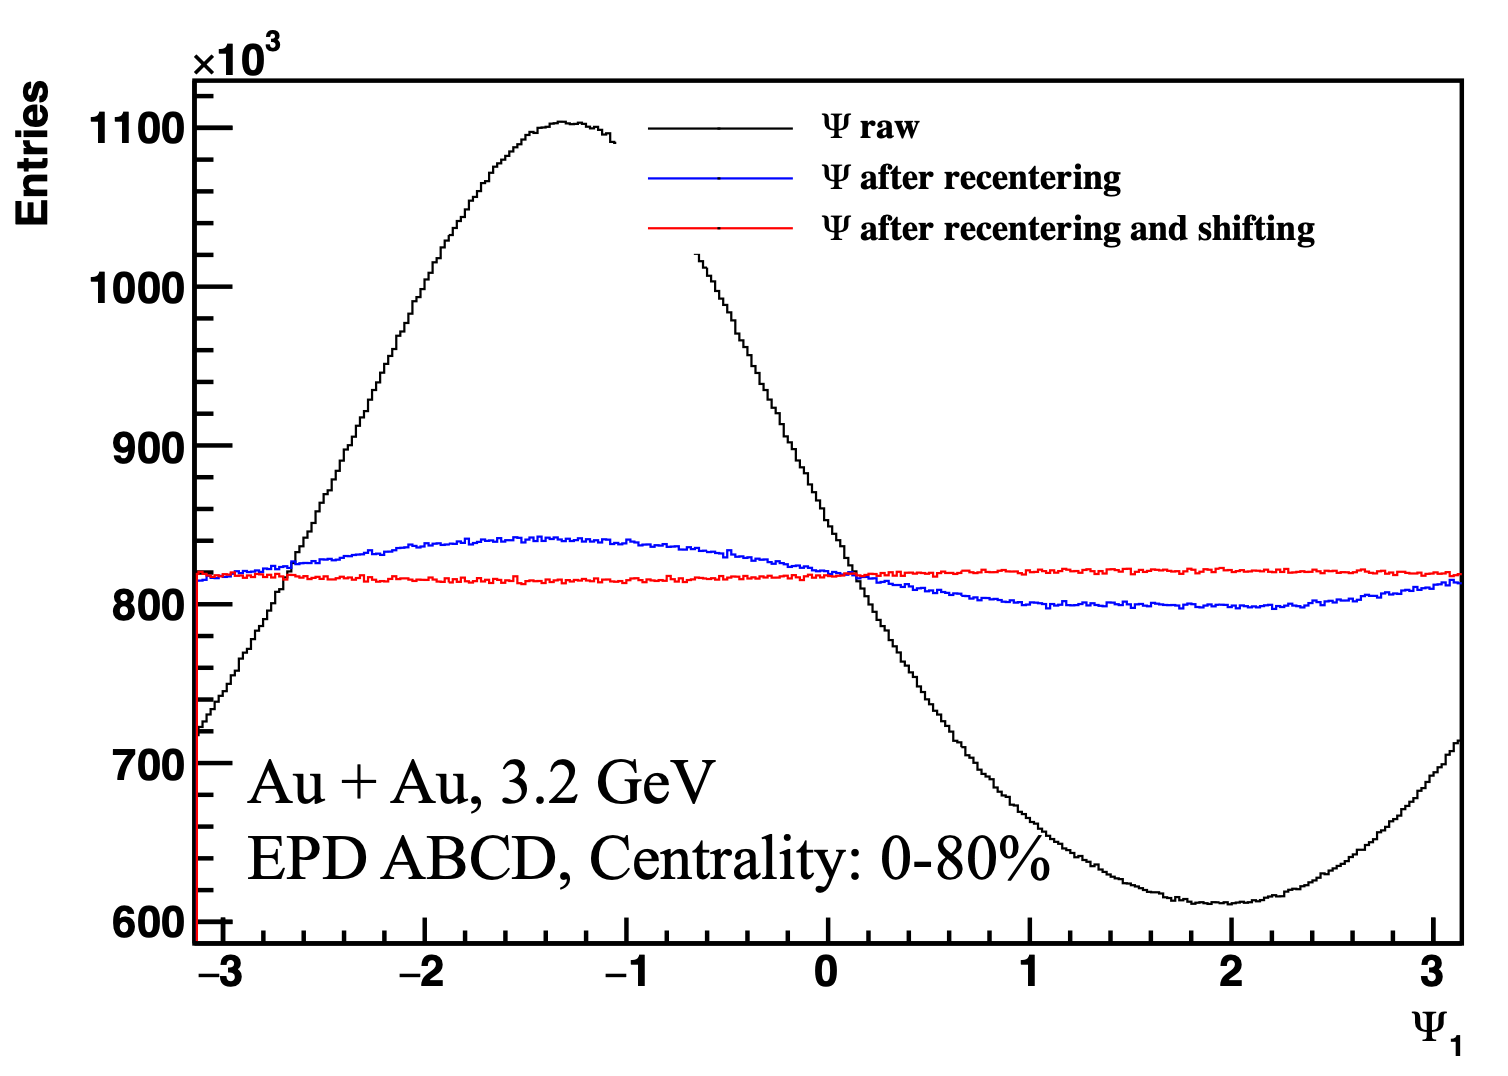
\includegraphics[width=0.45\linewidth]{figures/chapter02/EP_3p2GeV.png}
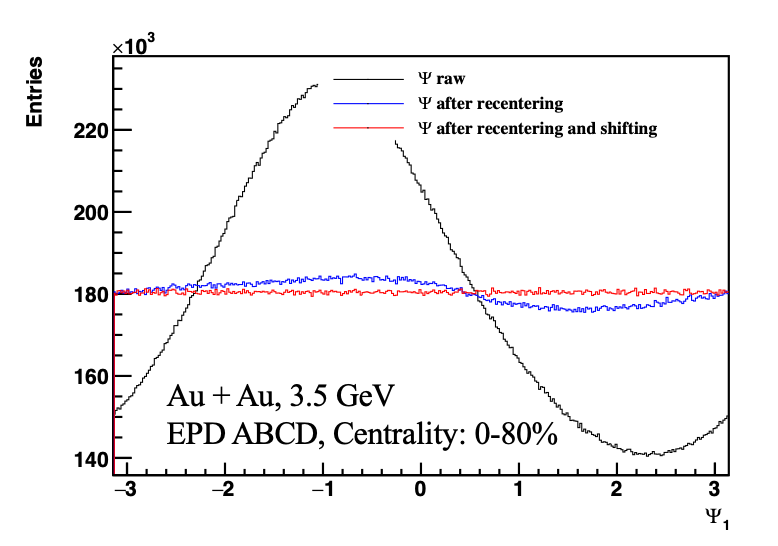
\includegraphics[width=0.45\linewidth]{figures/chapter02/EP_3p5GeV.png}
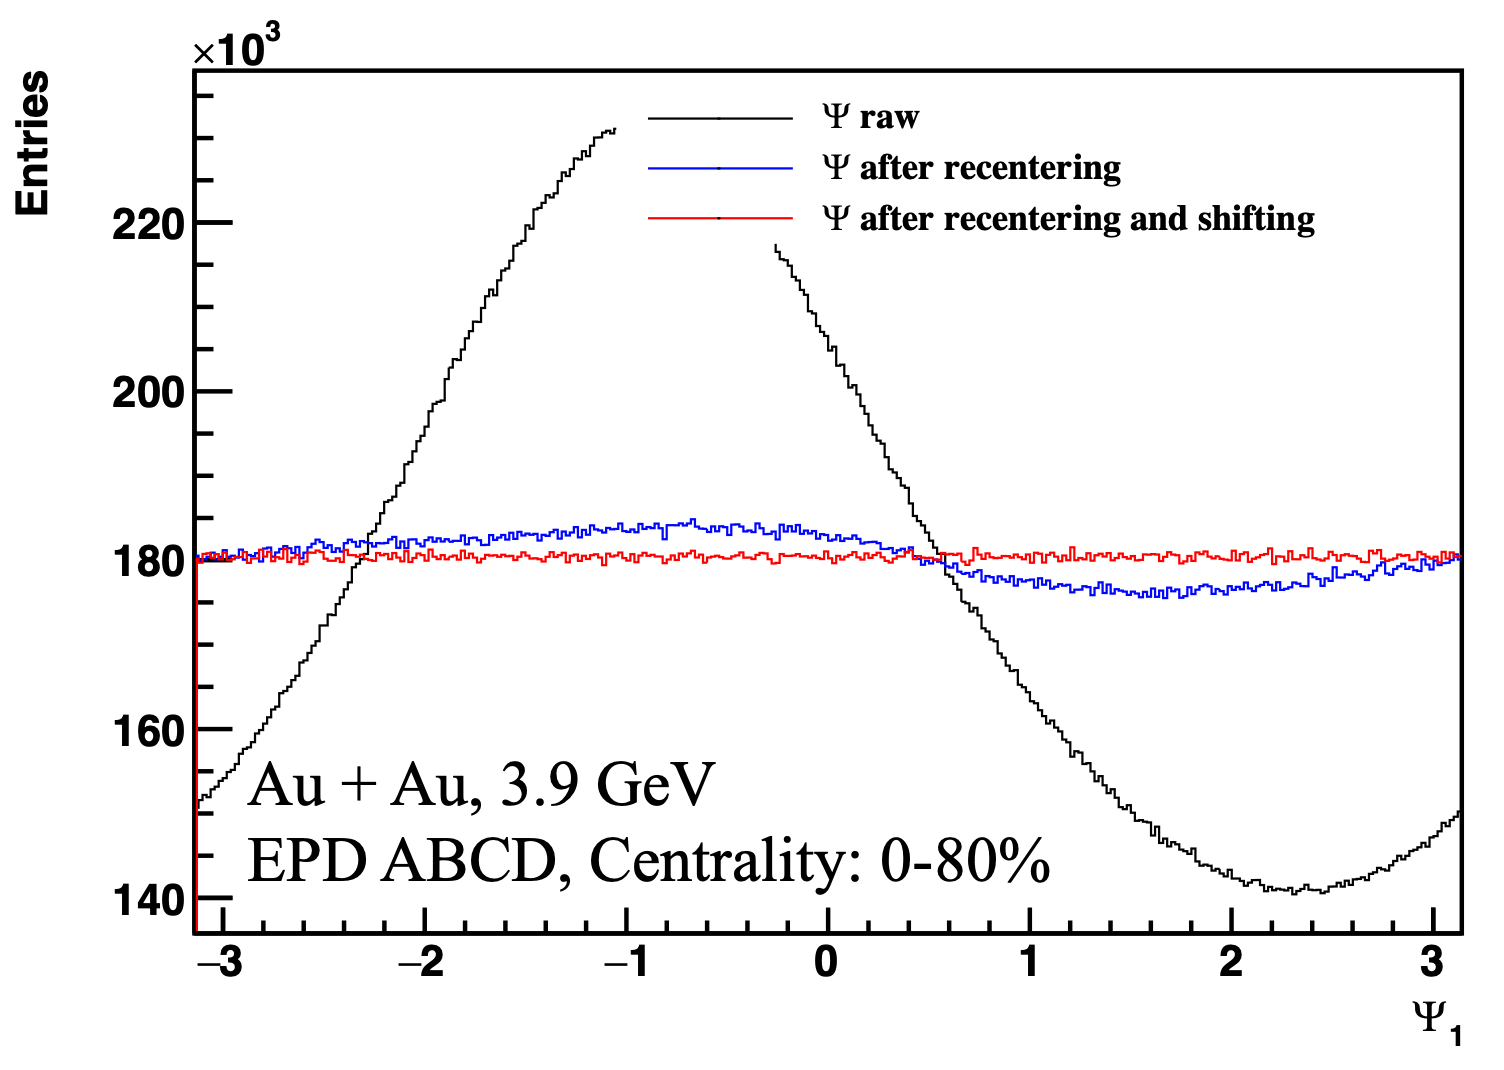
\includegraphics[width=0.45\linewidth]{figures/chapter02/EP_3p9GeV.png}
\caption{The event plane distribution on EPD.}
\label{fig:EP_distribution}
\end{figure}

\subsubsection{Event plane resolution}
After recentering and shifting calibration, the event plane is ready for the flow calculation. 
While the finite multiplicity in the experiment would limit the estimation of the reaction plane angle.~\cite{voloshin2008collective}
So the event plane resolution would be brought to correct the oberverd flow coefficients, which could be expressed as equation~\ref{eq:resolution}
\begin{equation}
R_n=\left\langle\cos \left[n\left(\Psi_n-\Psi_{\mathrm{r}}\right)\right]\right\rangle
\label{eq:resolution}
\end{equation}
Where $\Psi_r$ is reaction plane angle, $\Psi_n$ is the event plane angle.
The angle brackets denote averaging over many events. 

In the fixed target mode, one would not be able to get sub-events are equal, since the collision happens at 
the end of TPC. The resolution in different window are not equal, one need at least three windows to determine
the event plane resolution in each of them.~\cite{poskanzer1998methods} It could be expressed as
\begin{equation}
    \left\langle\cos \left(n\left(\Psi_m^a-\Psi_r\right)\right)\right\rangle=\sqrt{\frac{\left\langle\cos \left(n\left(\Psi_m^a-\Psi_m^b\right)\right)\right\rangle\left\langle\cos \left(n\left(\Psi_m^a-\Psi_m^c\right)\right)\right\rangle}{\left\langle\cos \left(n\left(\Psi_m^b-\Psi_m^c\right)\right)\right\rangle}}
\label{eq:threeSub_res}
\end{equation}
Where $\Psi_m^a$ is the target event plane angle,  $\Psi_m^b$ and  $\Psi_m^c$ are the reference event plane angle.

In this analysis, we foucus on directed flow($v_1$) measurement, they are both bashed on 
first order event plane. so we substitue $m=1$ to the equation~\ref{eq:threeSub_res}. According to the STAR published 3 GeV paper~\cite{Abdallah_2022},
One can get the largest resolution if chosen the forward eta window(EPD group A and B). We follow the method and take EPD group A and B 
as our target event plane. Other windows from EPD and TPC would be chosen as reference windows. They are divided as shown by Fig.~\ref{fig:EPD_TPC_groups}
This figure is specific for 3.0 GeV. We note here eta could reach 2.4 for 3.2, 3.5 and 3.9 GeV data, since inner TPC was upgarded at these three energies.
Two eta gaps were added in this analysis to reduce the non-flow effect. One eta gap is in the EPD group C which eta coverage is $[-3.3, -3.0]$(removed two EPD rings in C, here C' denotes group C after removing two rings), 
the other one is in the TPC which eta coverage is $[-1.1, -1.0]$ for 3GeV, while $[-1.15, -1.25]$ for 3.2, 3.5, and 3.9 GeV due to the wider eta coverage brought by iTPC. 
\begin{figure}[hbt!]
\centering
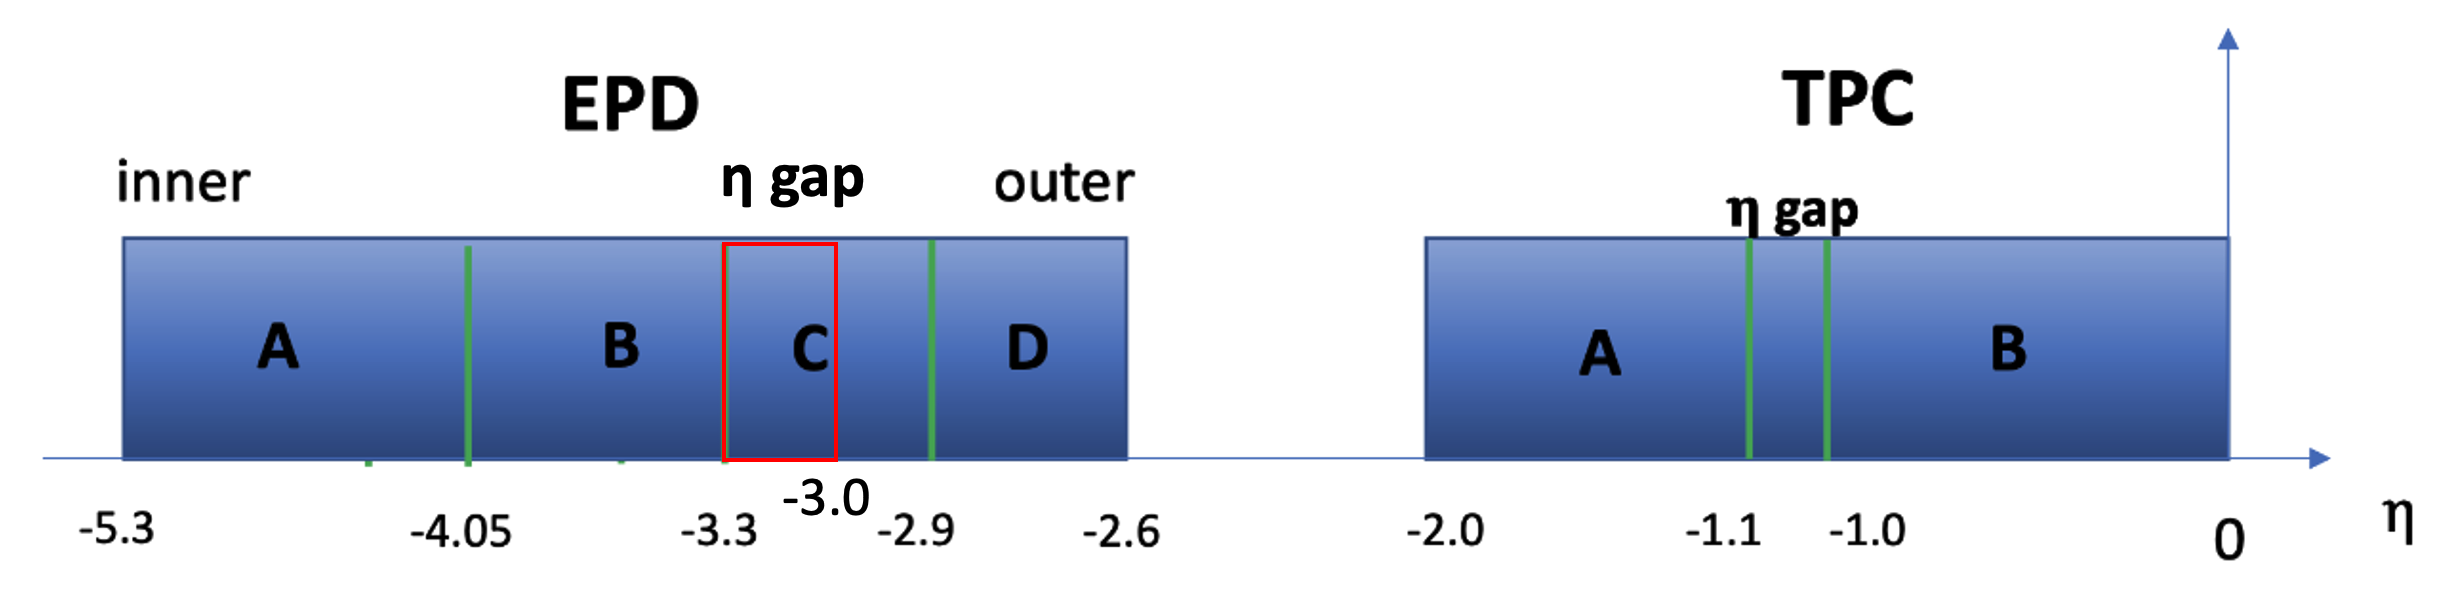
\includegraphics[width=0.65\linewidth]{figures/chapter02/EPD_TPC_groups.png}
\caption{The sketh of EPD and TPC groups.}
\label{fig:EPD_TPC_groups}
\end{figure}



The first order event plane resolution of EPD gourp AB at 3.0, 3.2, 3.5, and 3.9 GeV was show by Fig.~\ref{fig:1st_resolution}.
EPD group AB was chosen as the target event plane, and another two reference event plane were needed according to three sub-event plane method.
In this analysis, the maximum $R_1$(EPD-AB vs. EPD-C' and TPC-B) was chosen as default resolution to measure directed flow, which could be expressed as:
\begin{equation}
v_n=\frac{v_n^{\mathrm{obs}}}{R_n}
\label{eq:vn}
\end{equation}
The other two set of resolution were used to estimate the systematic uncertainty brought by resolution.

\begin{figure}[hbt!]
\centering
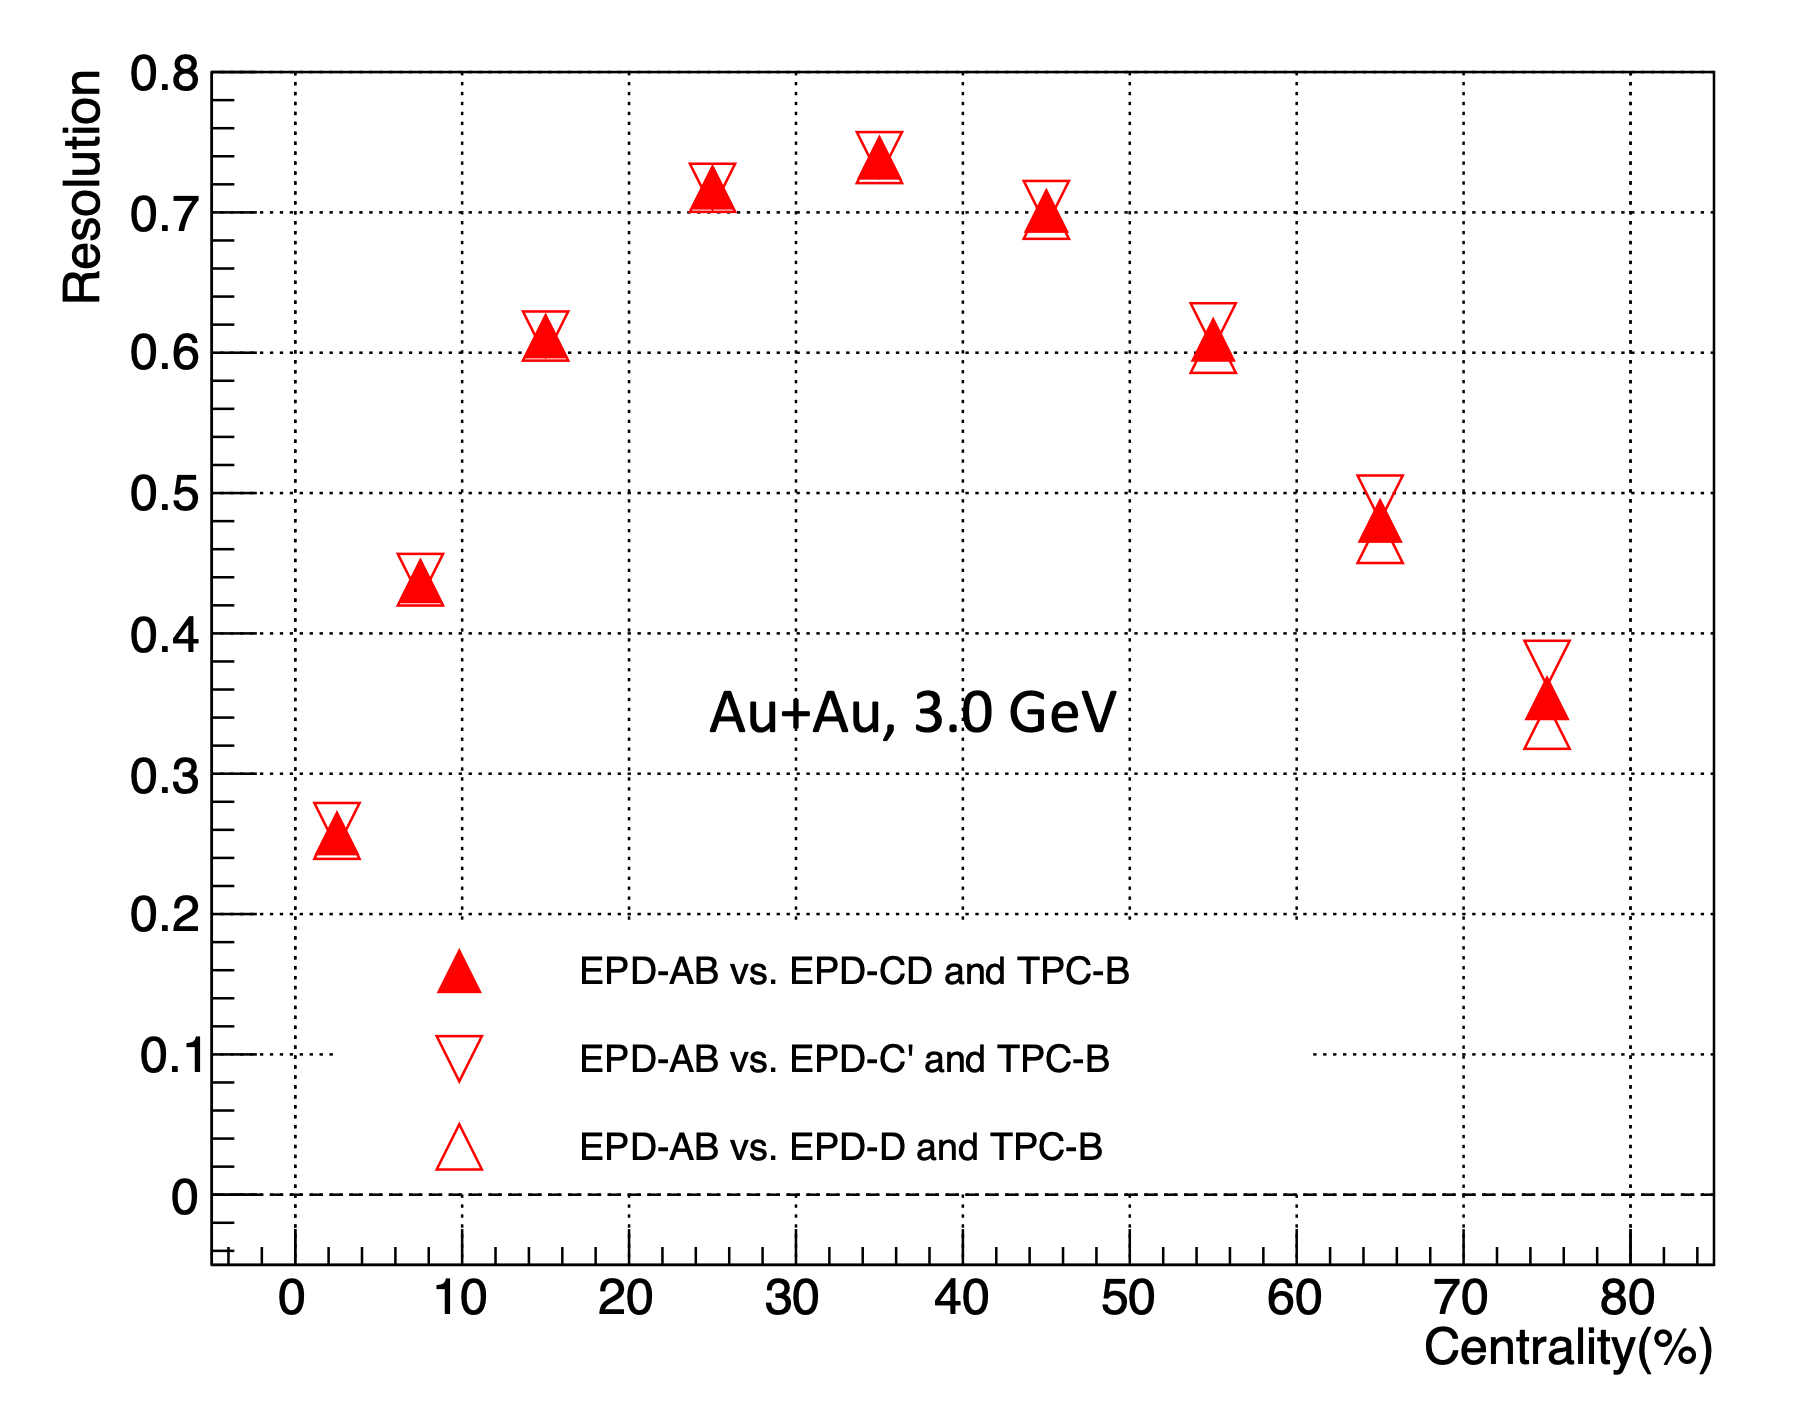
\includegraphics[width=0.45\linewidth]{figures/chapter02/res_3gev.png}
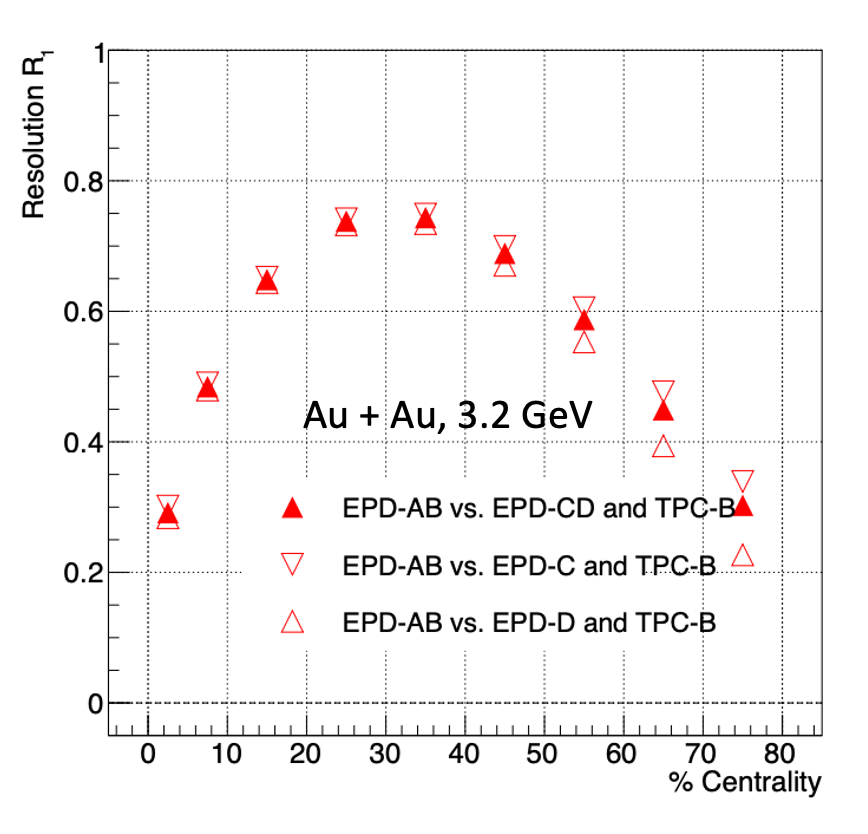
\includegraphics[width=0.40\linewidth]{figures/chapter02/res_3p2gev.png}
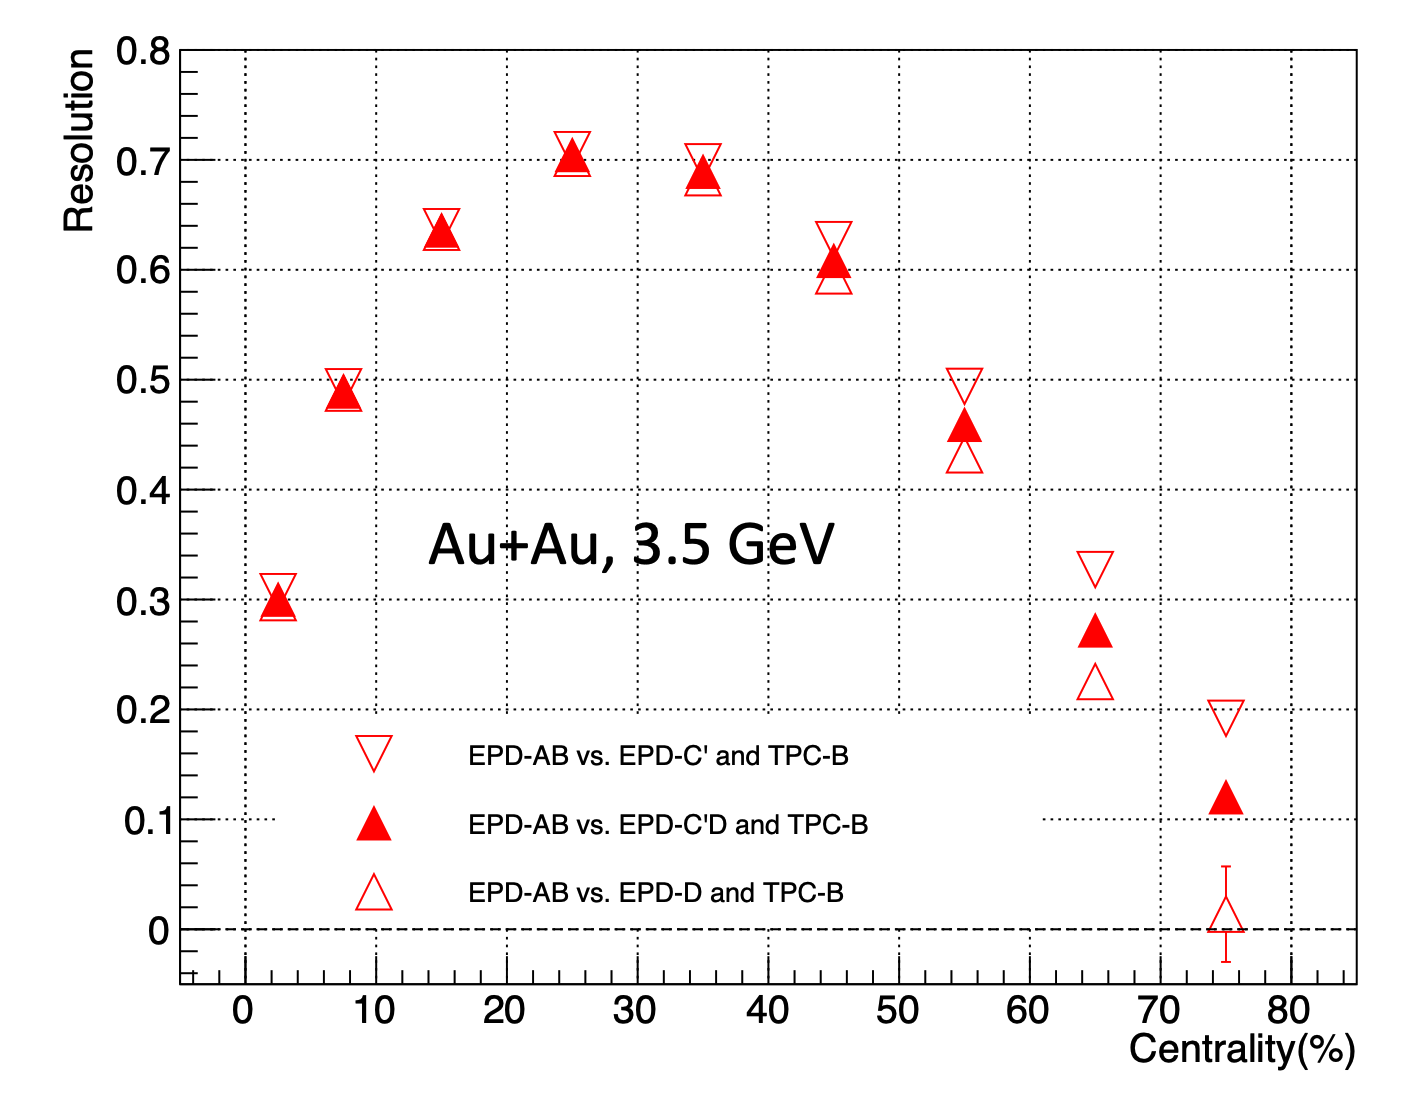
\includegraphics[width=0.45\linewidth]{figures/chapter02/res_3p5gev.png}
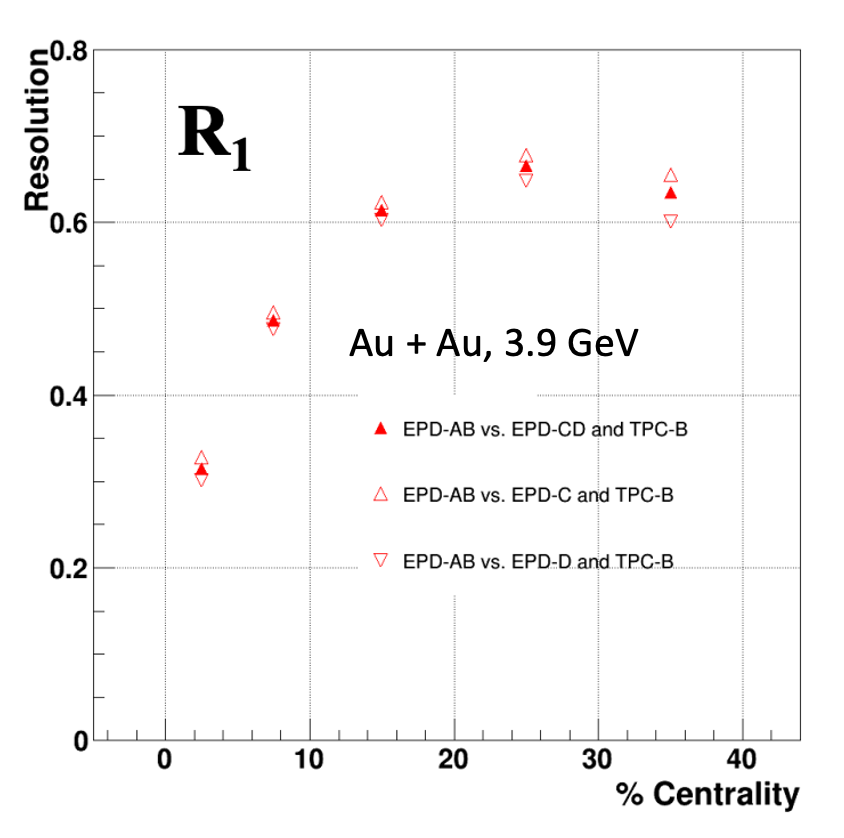
\includegraphics[width=0.40\linewidth]{figures/chapter02/res_3p9gev.png}
\caption{The first order event plane resolution of EPD gourp AB at 3.0, 3.2, 3.5, and 3.9 GeV.}
\label{fig:1st_resolution}
\end{figure}

\subsection{Particle identification}

\subsubsection{$\pi$, K, p identification}

Time Projection Chamber(TPC)\cite{ANDERSON2003659} and Time of Flight(TOF)\cite{LLOPE2012S110} were used to identify pion, kaon, and proton. 
The identification are based on particle ionization energy loss(dE/dx) in TPC and time of particle flight measured by TOF.
The theoretic particle ionization energy loss could be described by Bichsel function, which are shown by dashed line in left panel of Fig.~\ref{fig:dedx_m2}.
The dE/dx value would be transfored to $n\sigma_{particle}$ to facilitate applying the PID cut. The $n\sigma_{particle}$ can be expressed as:
\begin{equation}
n \sigma_{\text {particle }} \propto \ln \left[\left\langle\frac{d E}{d X}\right\rangle_{\text {particle }} /\left\langle\frac{d E}{d X}\right\rangle_{\text {Bichsel }}\right]
\label{eq:nsigma}
\end{equation}

In this analysis, we take the $n\sigma_{particle}$ shift into account which is due to detector issue and data calibration issue.
For example, the $n\sigma_{proton}$ distribution in momentum windows are shown by Fig.~\ref{fig:nsigmaproton_3p5}.
The background and signal peak were fitted with Gaussian function, and proton purity could reach more than 95\% up to momentum at 1.2 GeV/c.
At higer momentum region($p > 1.2 GeV/c$), the signal and background peak are merged, it's unable to assure proton purity greater than 95\% with TPC along.
In that case, TOF was involved to help identify particle at high momentum.

The right panel of Fig.~\ref{fig:dedx_m2} show rigidity dependence of mass square($m^2$) distribution measured by TOF, the $m^2$ could be calculated by the formula: 
$m^2 = p^2(1/\beta^2 - 1)$, where velocity $\beta = L/cT$. At hign momentum, we used $m^2$ distribution instead to study the particle purity. 
The $m^2$ distribution is after $n\sigma_{particle}$ cut from TPC. For example, Fig.~\ref{fig:m2_p_3p5} show proton $m^2$ distribution in momentum windows
after $|n\sigma_{proton} -shift| < 3$ cut. And Student-t function was applied to fit the signal peak and the background peak.
By that way, proton identification could reach p = 4.2 GeV/c, and the purity is greater than 95\%. Purity of pion and kaon is greater than 95\% and 90\%, respectively.  
The detailed PID cuts are shown by the TABLE~\ref{tab:pid_piKp} in the appendix for 3, 3.2, 3.5, and 3.9 GeV.

The accaptance of $\pi, K, p$ at 3.5 GeV are shown by Fig.~\ref{fig:3p5_piKp_acceptance}, the black box show the measured arear, where the rapdity cut is $-1<y_{CM}<0$, 
and $p_T$ cut are $0.2<p_T<1.6, 0.4<p_T<2.0$ for $\pi$/K, proton, respectively. For other energies, 3(Fig.~\ref{fig:3gev_piKp_acceptance}), 3.2, and 3.9 GeV, the acceptance plots could be found in the appendix. 

\begin{figure}[hbt!]
\centering
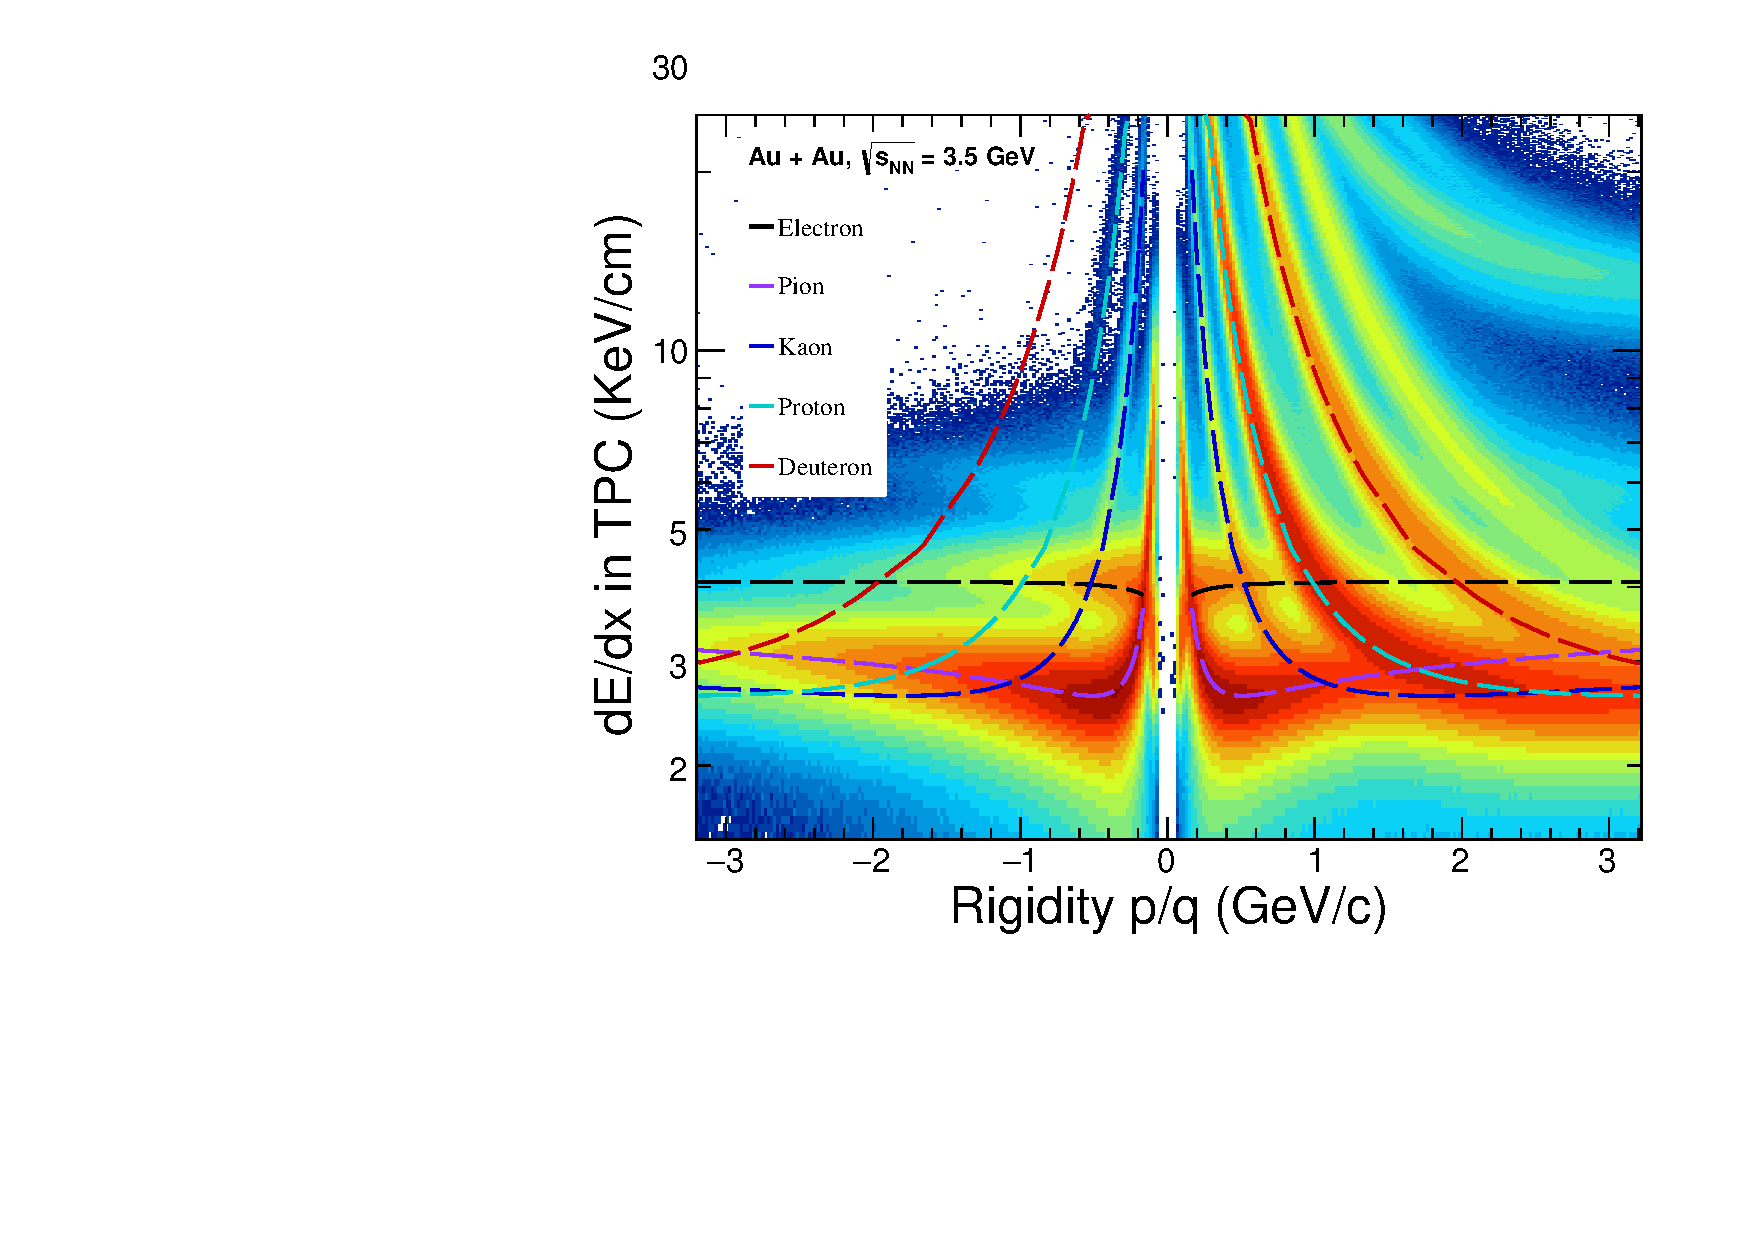
\includegraphics[width=0.35\linewidth]{figures/chapter02/3p5GeV_dEdx_P23id.pdf}
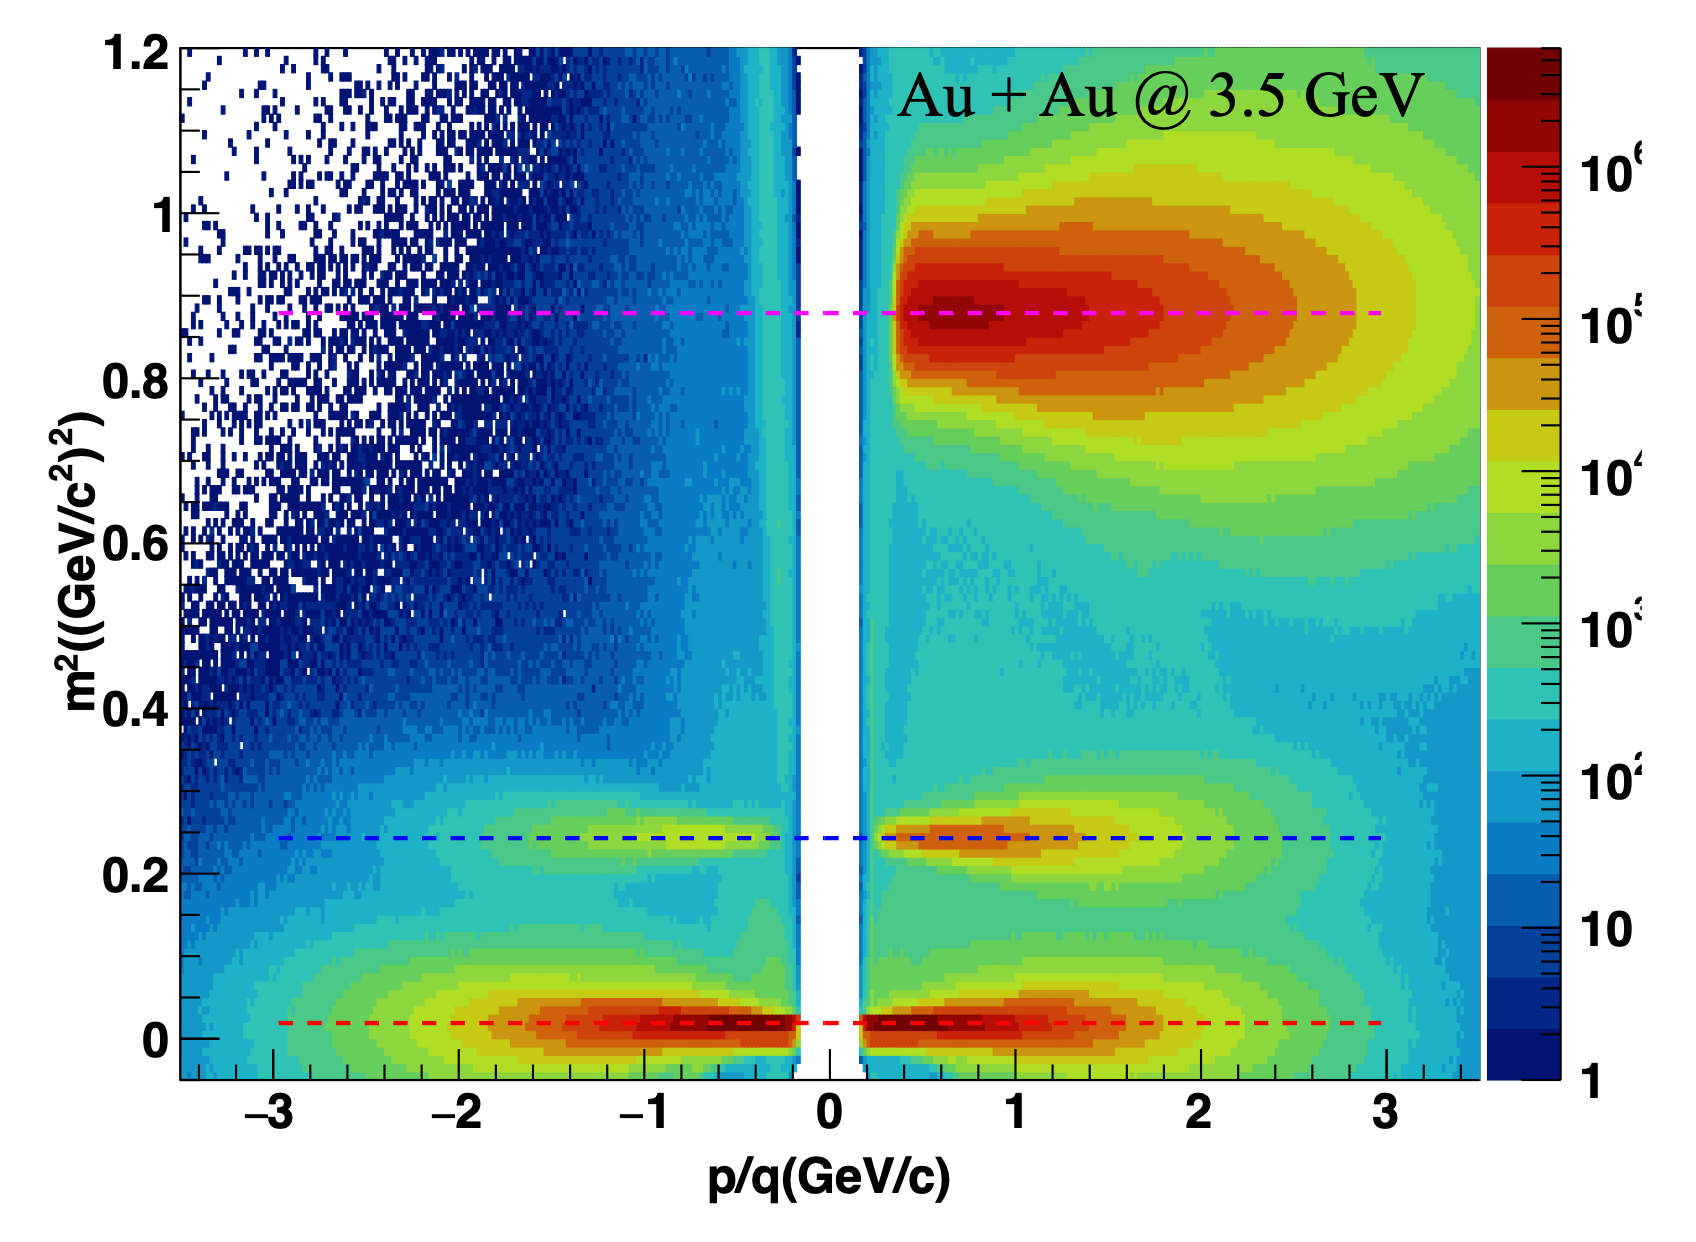
\includegraphics[width=0.35\linewidth]{figures/chapter02/m2_3p5gev.png}
\caption{Left: rigidity dependence of particle ionization energy loss in TPC, Right: rigidity dependence of particle mass square distribution measured by TOF in Au + Au collisions at $\sqrt{s_{NN}}$ = 3.5 GeV.}
\label{fig:dedx_m2}
\end{figure}

\begin{figure}[hbt!]
\centering
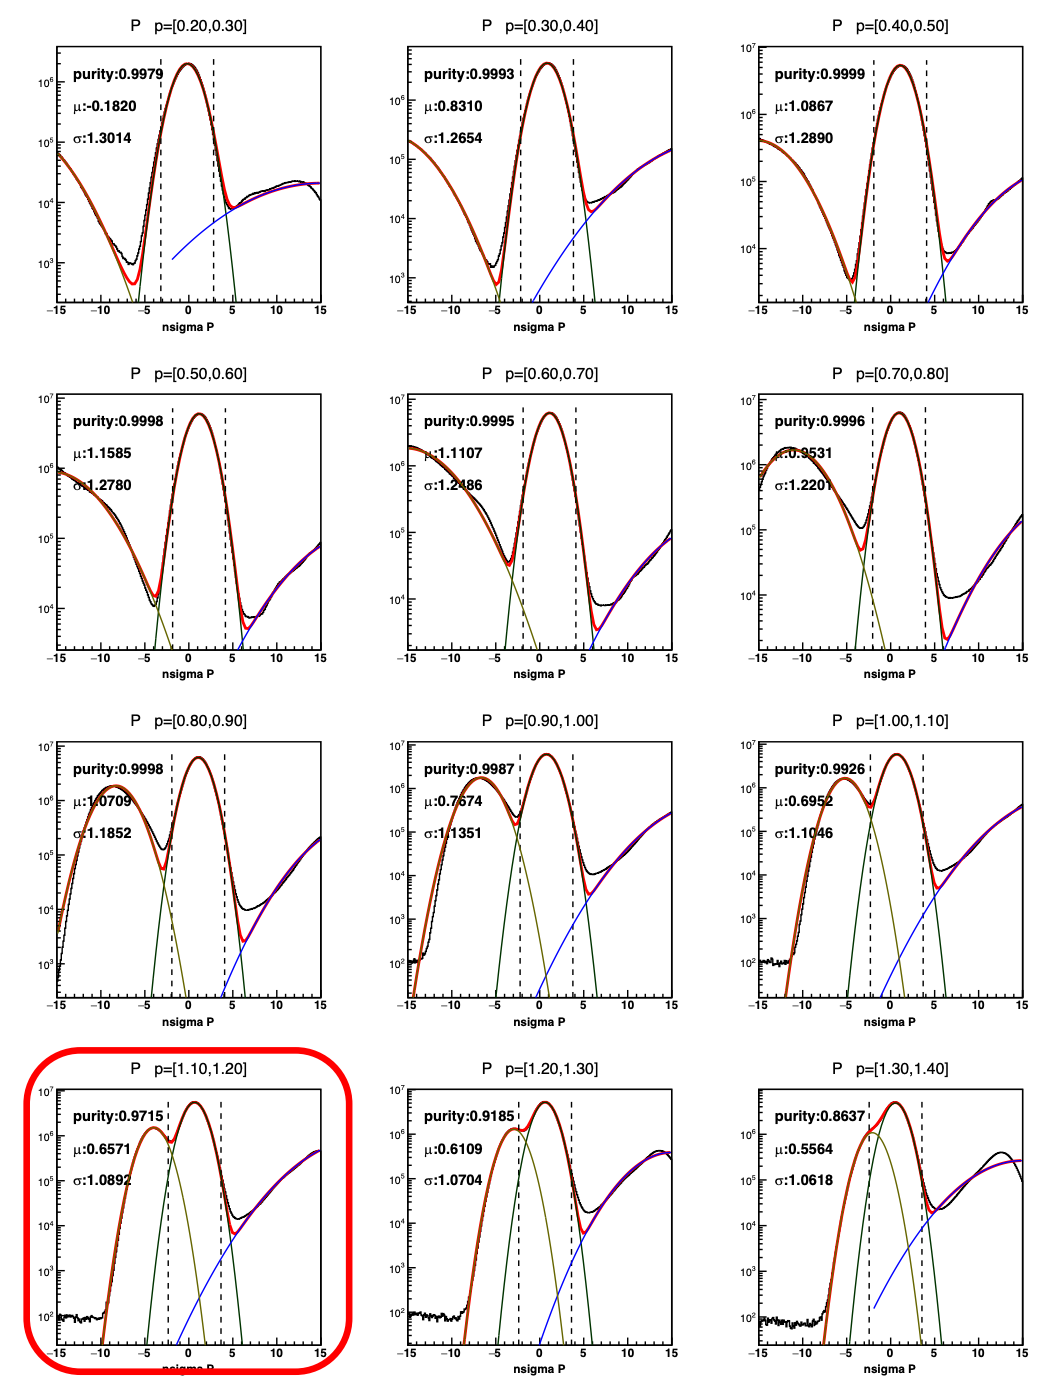
\includegraphics[width=0.55\linewidth]{figures/chapter02/nsigmaproton_3p5gev.png}
\caption{$n\sigma_{proton}$ distribution in momentum windows from TPC at $\sqrt{s_{NN}}$ = 3.5 GeV.}
\label{fig:nsigmaproton_3p5}
\end{figure}

\begin{figure}[hbt!]
\centering
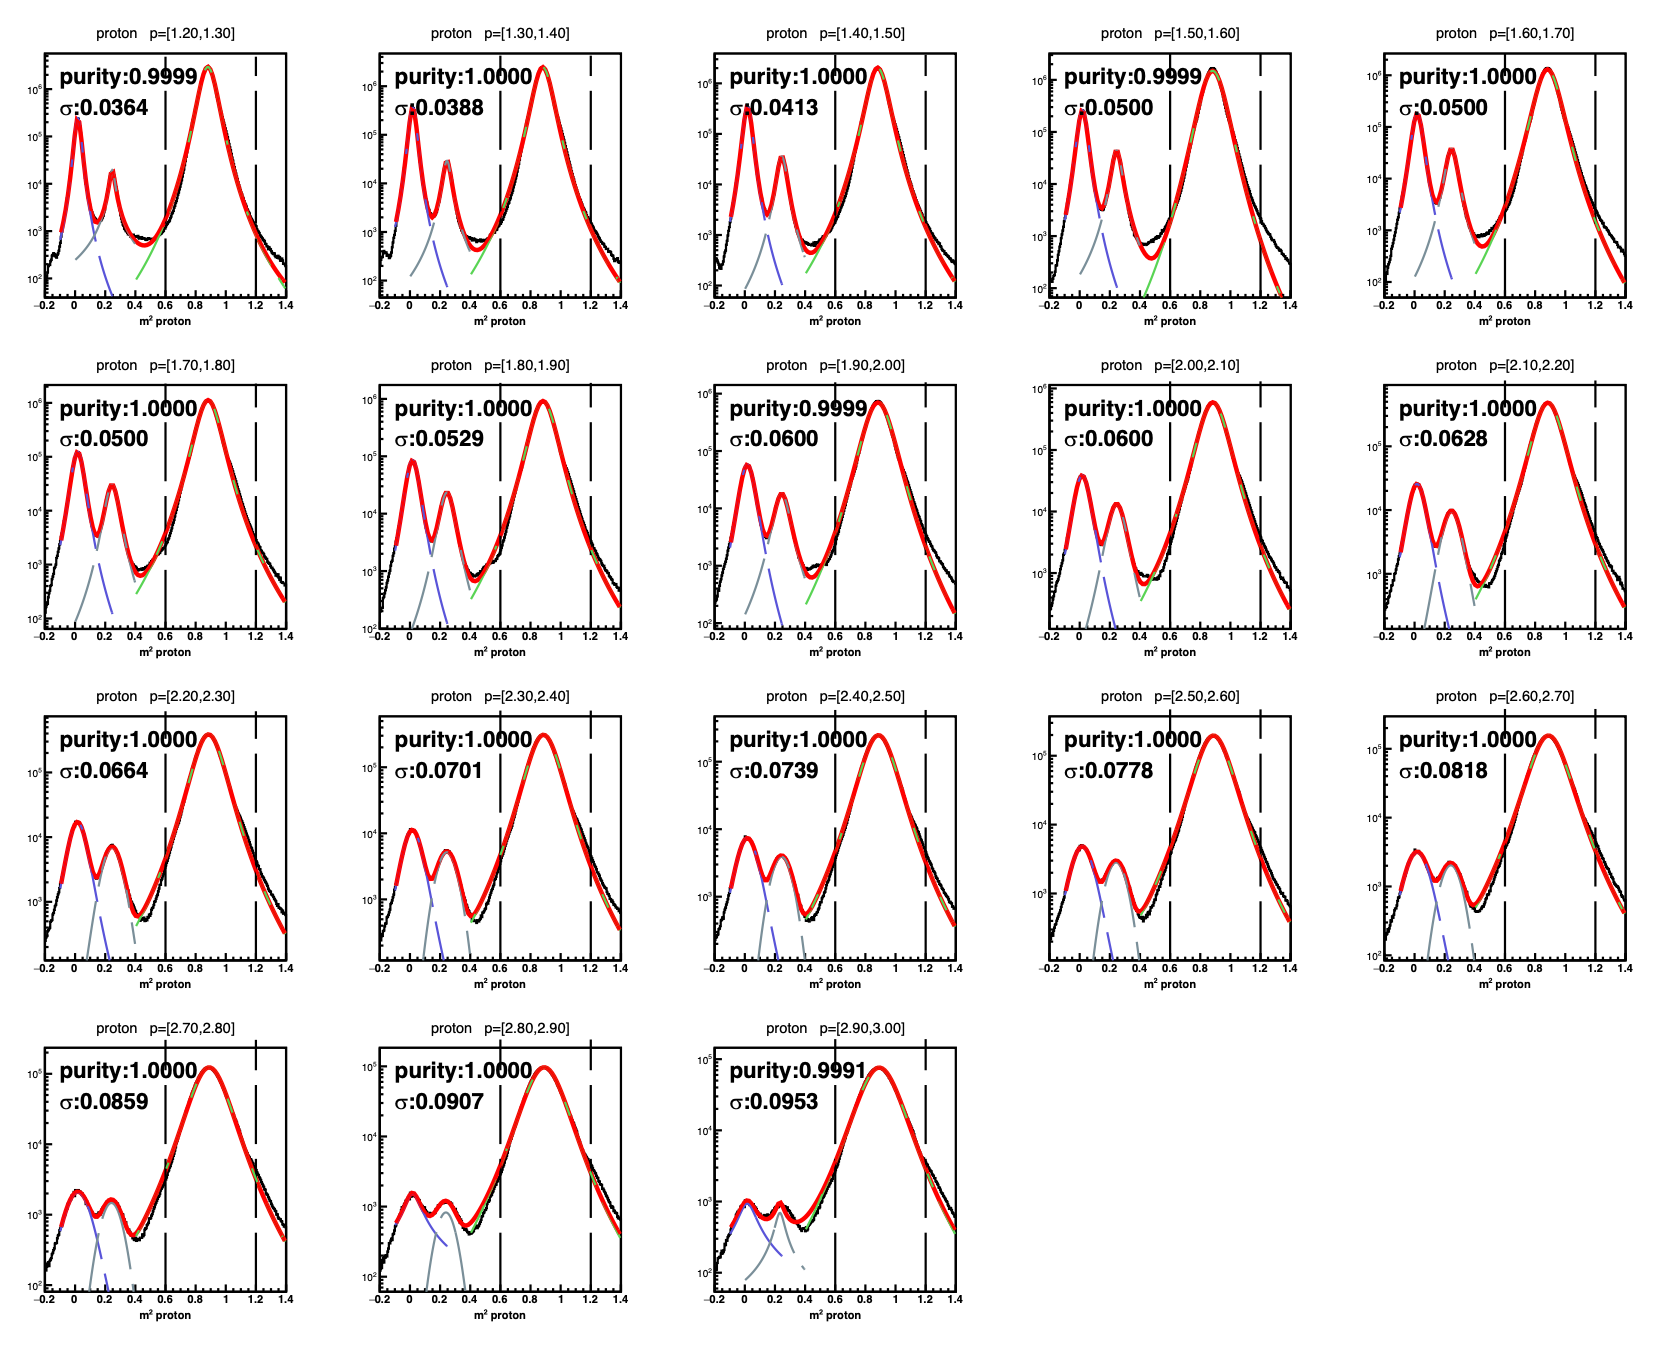
\includegraphics[width=0.55\linewidth]{figures/chapter02/m2_p_3p5gev.png}
\caption{$m^2$ distribution in momentum windows from TOF at $\sqrt{s_{NN}}$ = 3.5 GeV.}
\label{fig:m2_p_3p5}
\end{figure}

\begin{figure}[hbt!]
\centering
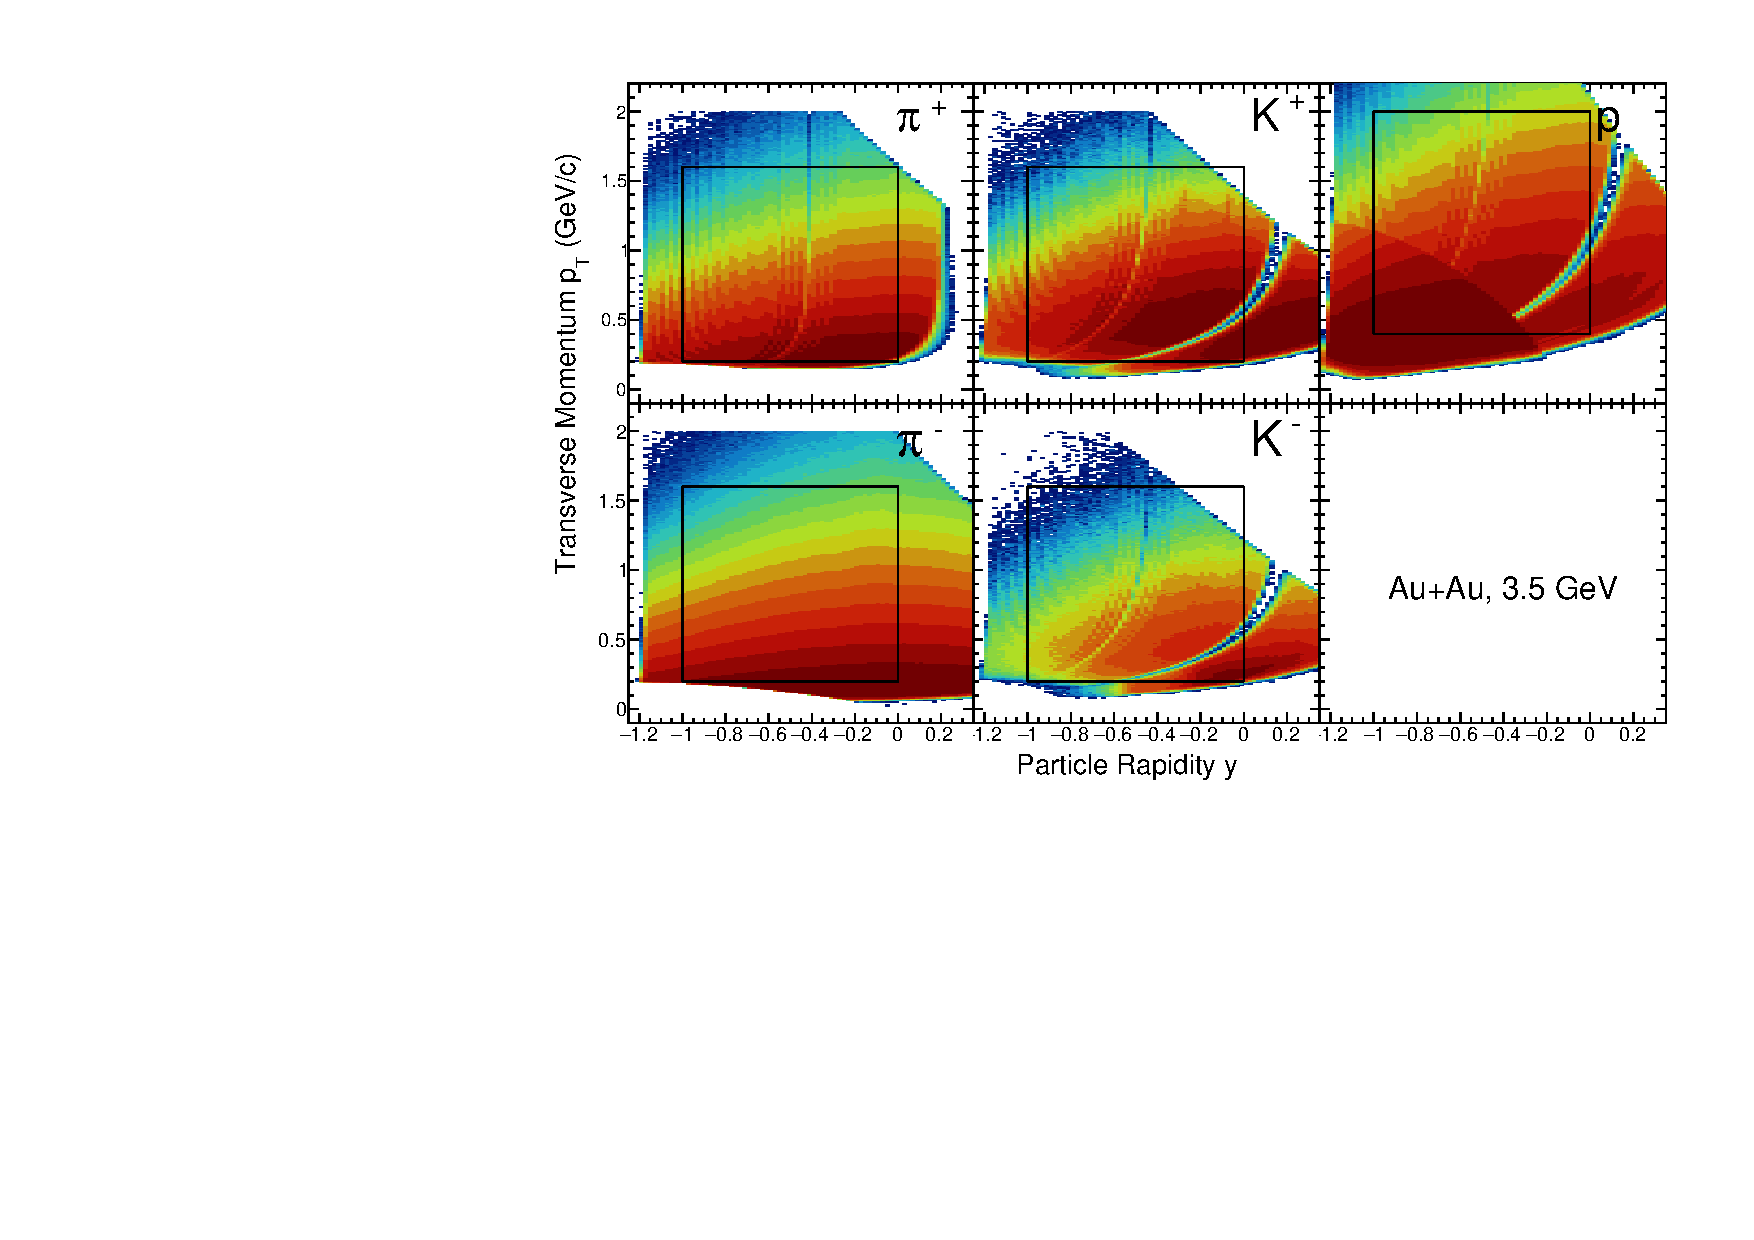
\includegraphics[width=0.55\linewidth]{figures/chapter02/3p5_piKp_acceptance.pdf}
\caption{$\pi, K, p$ density distribution as function of rapidity and transverse momentum at $\sqrt{s_{NN}}$ = 3.5 GeV.}
\label{fig:3p5_piKp_acceptance}
\end{figure}


\subsubsection{$K^{0}_{S}, \Lambda$ identification}

For the weak decay particles $K^{0}_{S}~and~\Lambda$, they are reconstructed by Kalman Filter(KF) particle package\cite{doi:10.1142/S0217751X20430034},
where the covariance matrix of reconstructed tracks are considered to construct a set of topological variable.
The track and topological cuts for daughters are listed in the TABLE.~\ref{tab:K0s_lam_cut}.
Note that only $\pi^{+}$ was required to have $m^2$ cut to avoid contamination from proton.

\begin{table}
    \centering
    \begin{tabular}{|c|c|c|l|l|l|} \hline 
         Daughters' track cuts&  $nHitsFit > 15$ &\makecell{$|n\sigma_{\pi,p}-shift| < 3$, \\$\pi^{+}: -0.06 < m^2 < 0.1$}&$0.04 < Error(dE/dx ) < 0.12$ &$nHitsdEdx > 5$\\ \hline 
         Topological cuts&  $\chi^2_{prim, \pi}<10$&   $\chi^2_{prim, p}<10$& &\\ \hline
    \end{tabular}
    \caption{Daughters' track cuts and topological cuts applied for $K^{0}_{S}, \Lambda$ in KF particle}
    \label{tab:K0s_lam_cut}
\end{table}
The acceptance of $K^{0}_{S}~and~\Lambda$ are shown by Fig.~\ref{fig:3p5_K0s_lambda_acceptance}. 
The black box show the kinematic region chosen in this analysis, where the rapdity cut is $-1<y_{CM}<0$, 
and $p_T$ cut are $0.2<p_T<1.6, 0.4<p_T<2.0$ for $K^{0}_{S} and \Lambda$, respectively.
The accaptance plots could be found in the appendix for other energies(3GeV(Fig.~\ref{fig:3gev_K0s_lambda_acceptance}), 3.2 GeV, 3.9 GeV).



\begin{figure}[hbt!]
\centering
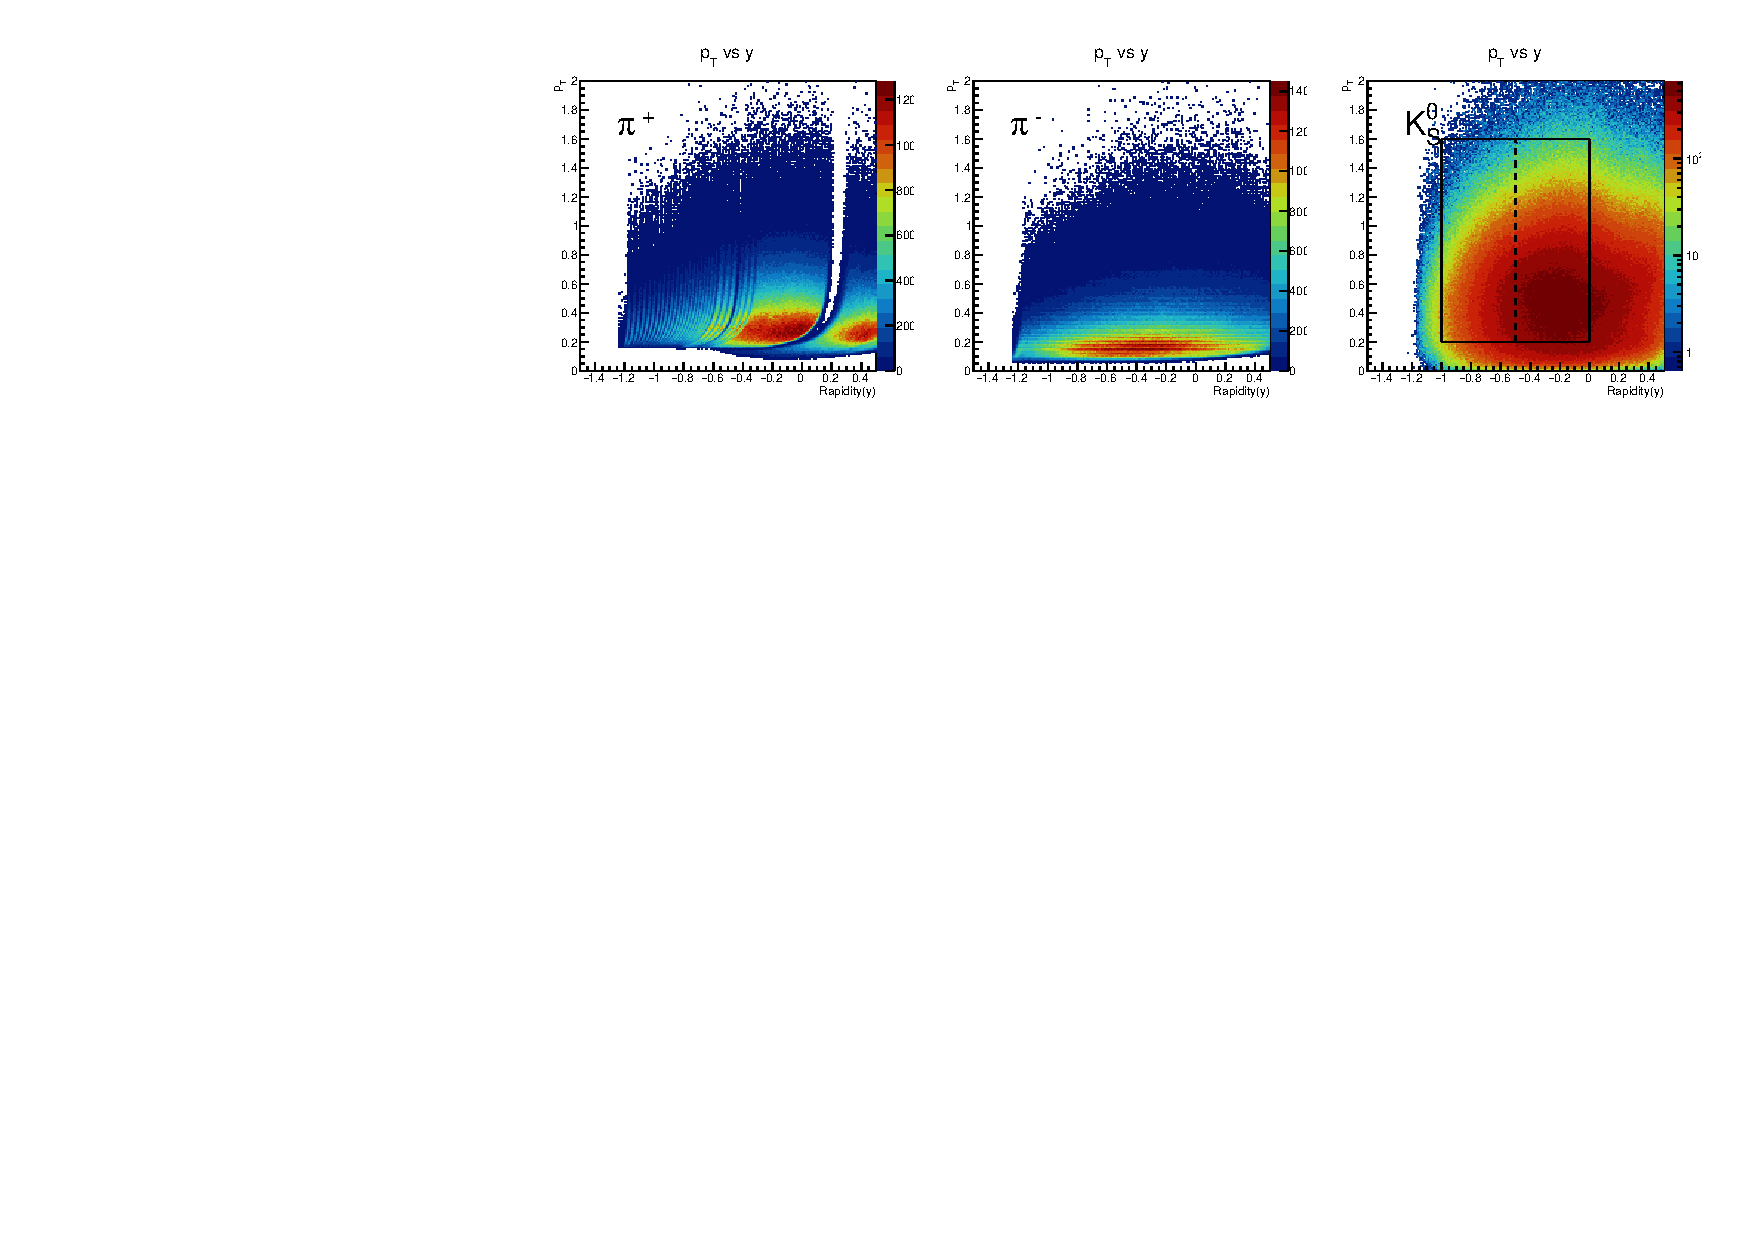
\includegraphics[width=0.55\linewidth]{figures/chapter02/3p5gev_K0s_acceptance.pdf}
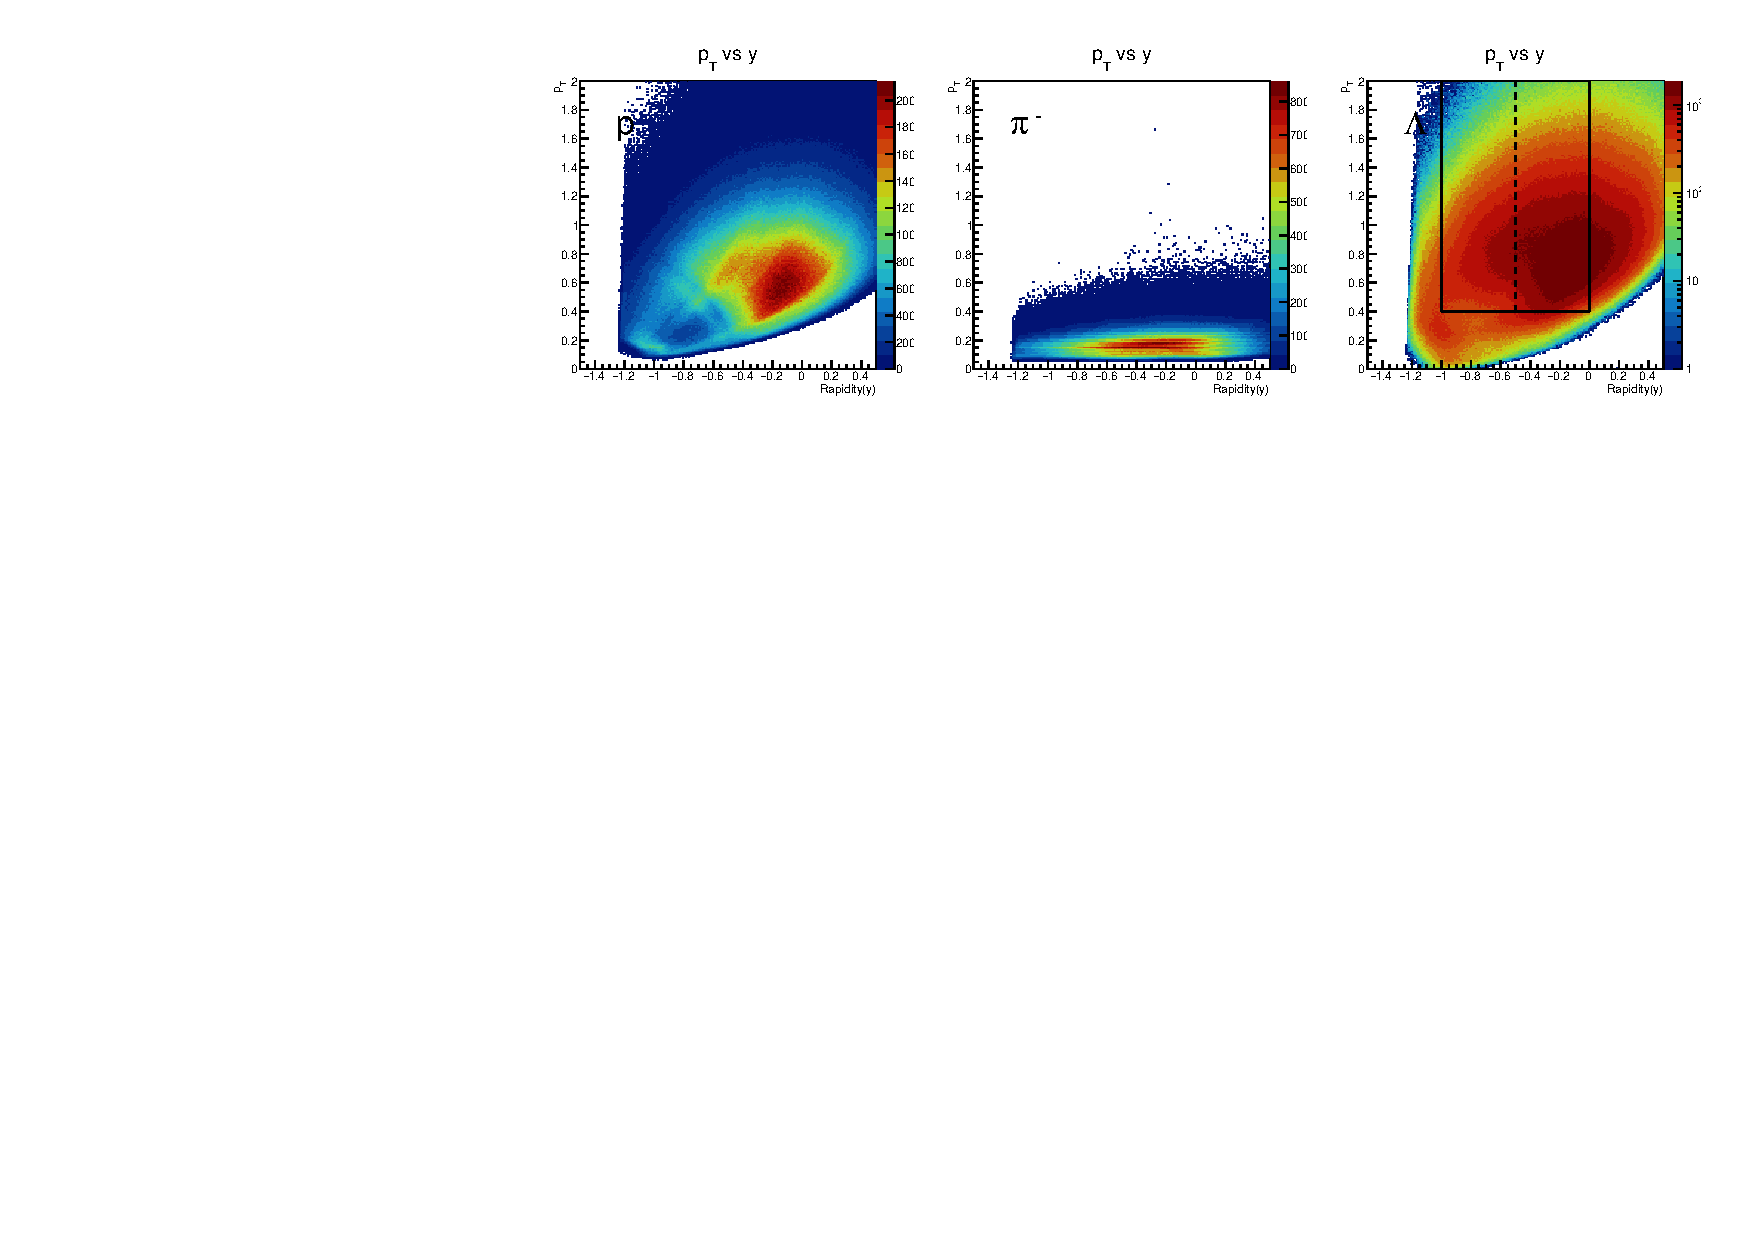
\includegraphics[width=0.55\linewidth]{figures/chapter02/3p5gev_lambda_acceptance.pdf}
\caption{$K^{0}_{S}~and~\Lambda$(and their daughters) density distribution as function of rapidity and transverse momentum at $\sqrt{s_{NN}}$ = 3.5 GeV.}
\label{fig:3p5_K0s_lambda_acceptance}
\end{figure}



\subsection{Efficiency correction}


The efficiency correction would help to restore the particle which was not tracked by the detector.
In this analysis, TPC tracking efficiency and TOF matching efficiency are taken into account for $\pi, K, and p.$
For the weak decay particles($K^{0}_{S}~and~\Lambda$) which are reconstructed by KF particle package, 
the reconstruction efficiency was applied instead. 

The GEANT model\cite{AGOSTINELLI2003250} was used to simulate particle going through the detector based on Monte Carlo method, 
which could estimate the particle number loss due to the detector accaptance and the efficiency of reconstructing particle track.
For $K^0_S~and~\Lambda$, the GEANT model can also estimate the particle reconstruction efficiency.

The TPC tracking efficiency as function of rapidity and transverse momentum could be obtained by the formula~\ref{eq:tpc_eff}
\begin{equation}
    \epsilon_{TPC}\left(p_T, y\right)=\frac{\text {Number of Real Tracks }}{\text { Number of MC Tracks }}
\label{eq:tpc_eff}
\end{equation}
The embedding data used in this analysis could be found at the RCF: \\
\verb|/star/u/xgn1992/Strangeness/Phi/3p85GeV_fixTarget/SL19e/Simulation/Embedding| for 3 GeV,
\verb|/star/data105/embedding/production_4p59_fixedTarget_2019| for 3.2 GeV.

The TPC tracking efficiency for $\pi, K, p$ are shown by Fig.~\ref{fig:3p2_piKp_TPCeff} at 3.2 GeV. 
The black box show the measured rapdity and transverse momentum interval, where the rapdity cut is $-1<y_{CM}<0$, 
and $p_T$ cut are $0.2<p_T<1.6, 0.4<p_T<2.0$ for $\pi/K ~and~ p$, respectively. 
For other energies, the TPC tracking efficiency can be found in the appendix.(3GeV(Fig~\ref{fig:3gev_piKp_TPCeff}), 3.5GeV, 3.9GeV)

\begin{figure}[hbt!]
\centering
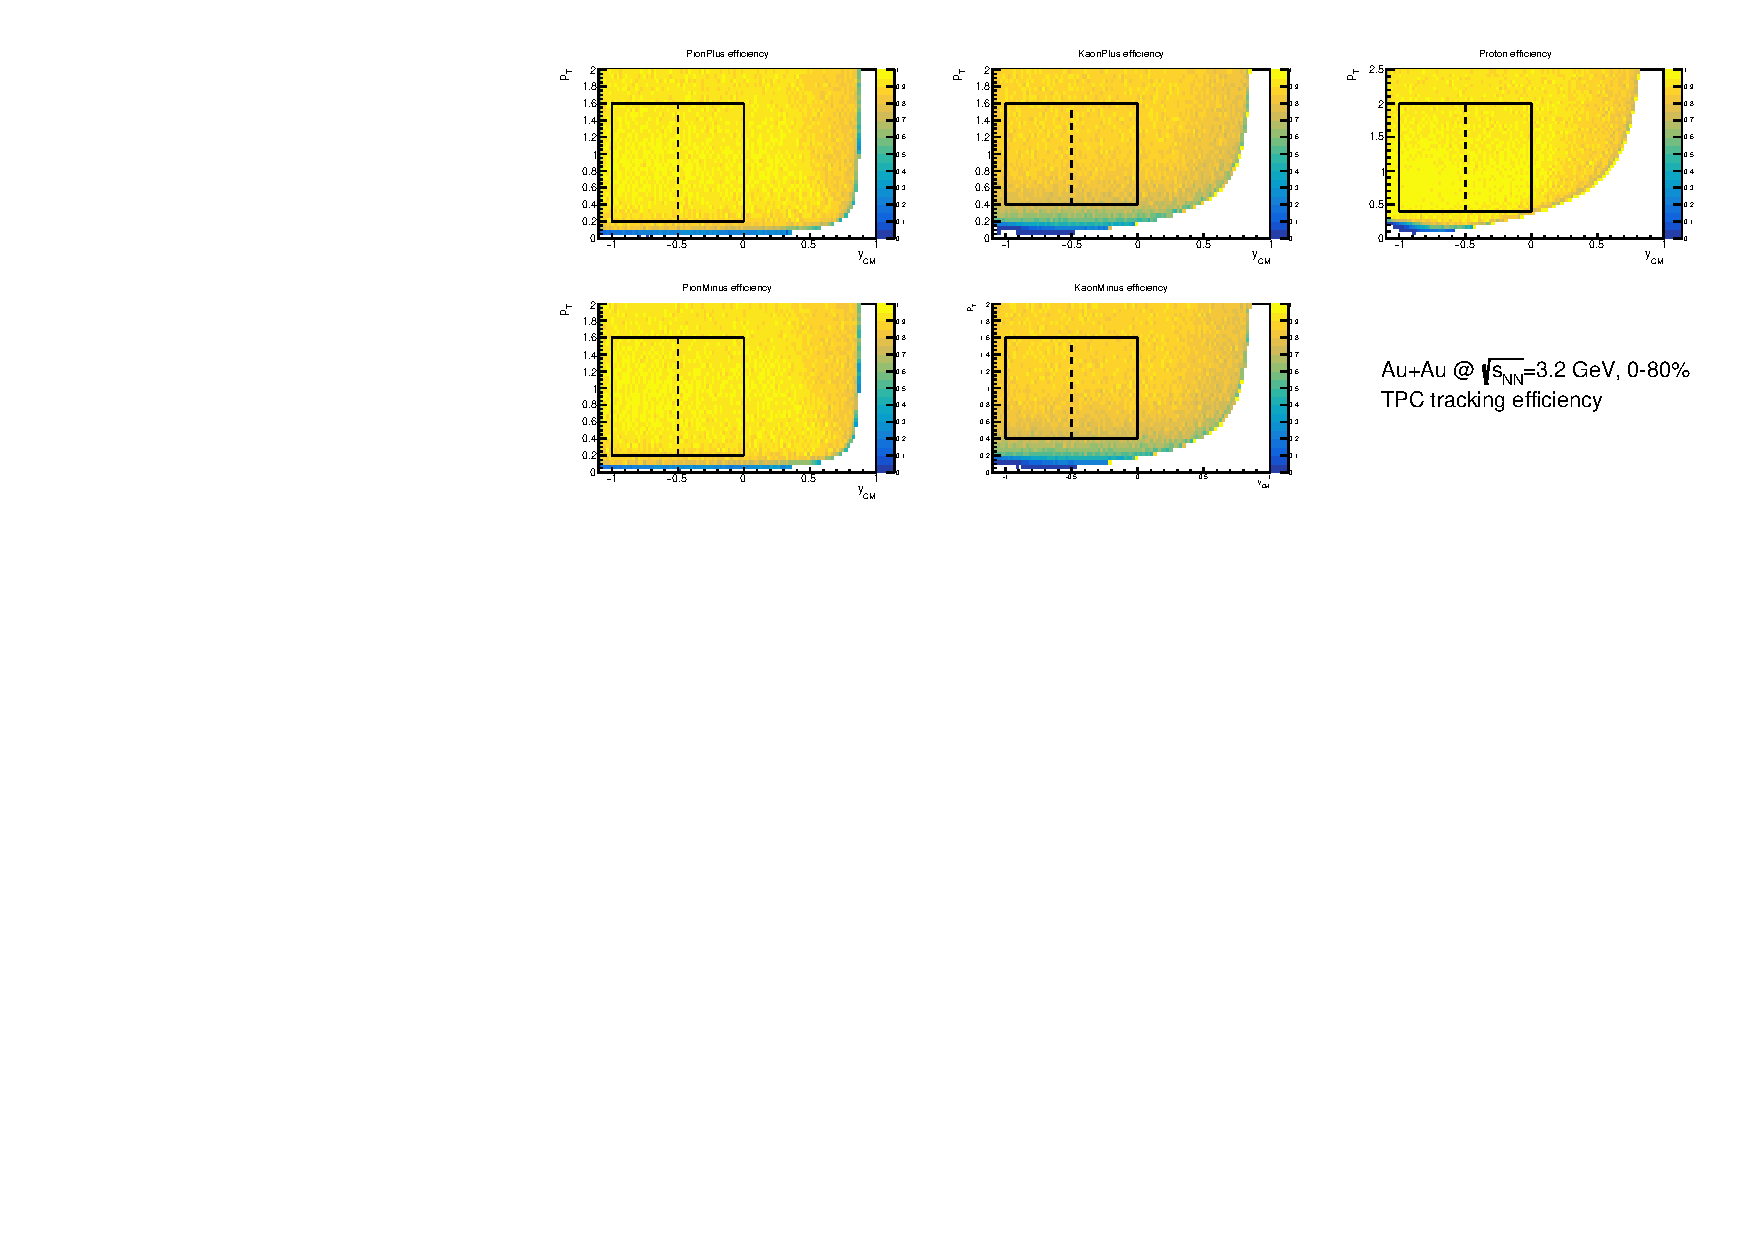
\includegraphics[width=0.65\linewidth]{figures/chapter02/3p2gev_TPC_eff.pdf}
\caption{TPC tracking efficiency of $\pi, K, p$ as function of rapidity y and transverse momentum $p_T$ at $\sqrt{s_{NN}}$ = 3.2 GeV.}
\label{fig:3p2_piKp_TPCeff}
\end{figure}

The TOF can improve the particle identification capability at high momentum region, 
which is necessary for kaon identification, discussed in the PID section.
While some particles which have tracks in TPC can not travel into TOF, and are not recorded by TOF.
The TOF matching efficiency could compensate to the un-recorded part, 
which can be expressed by the formula~\ref{eq:tof_eff}. Note that TPC tracks are required within $|n\sigma_{particle}-shift|<3$,
and TOF tracks just are required the TOF match flag is greater than zero.
\begin{equation}
    \epsilon_{TPC}\left(p_T, y\right)=\frac{\text {Number of TOF Tracks }}{\text { Number of TPC Tracks }}
\label{eq:tof_eff}
\end{equation}
The TOF matching efficiency for $\pi, K, p$ are shown by Fig.~\ref{fig:3p2_piKp_TOFeff} at 3.2 GeV. 
The black box show the measured rapdity and transverse momentum interval, where the rapdity cut is $-1<y_{CM}<0$, 
and $p_T$ cut are $0.2<p_T<1.6, 0.4<p_T<2.0$ for $\pi/K ~and~ p$, respectively. 
For other energies, the TOF matching efficiency can be found in the appendix.(3GeV(Fig~\ref{fig:3gev_piKp_TOFeff}), 3.5GeV, 3.9GeV)
\begin{figure}[hbt!]
\centering
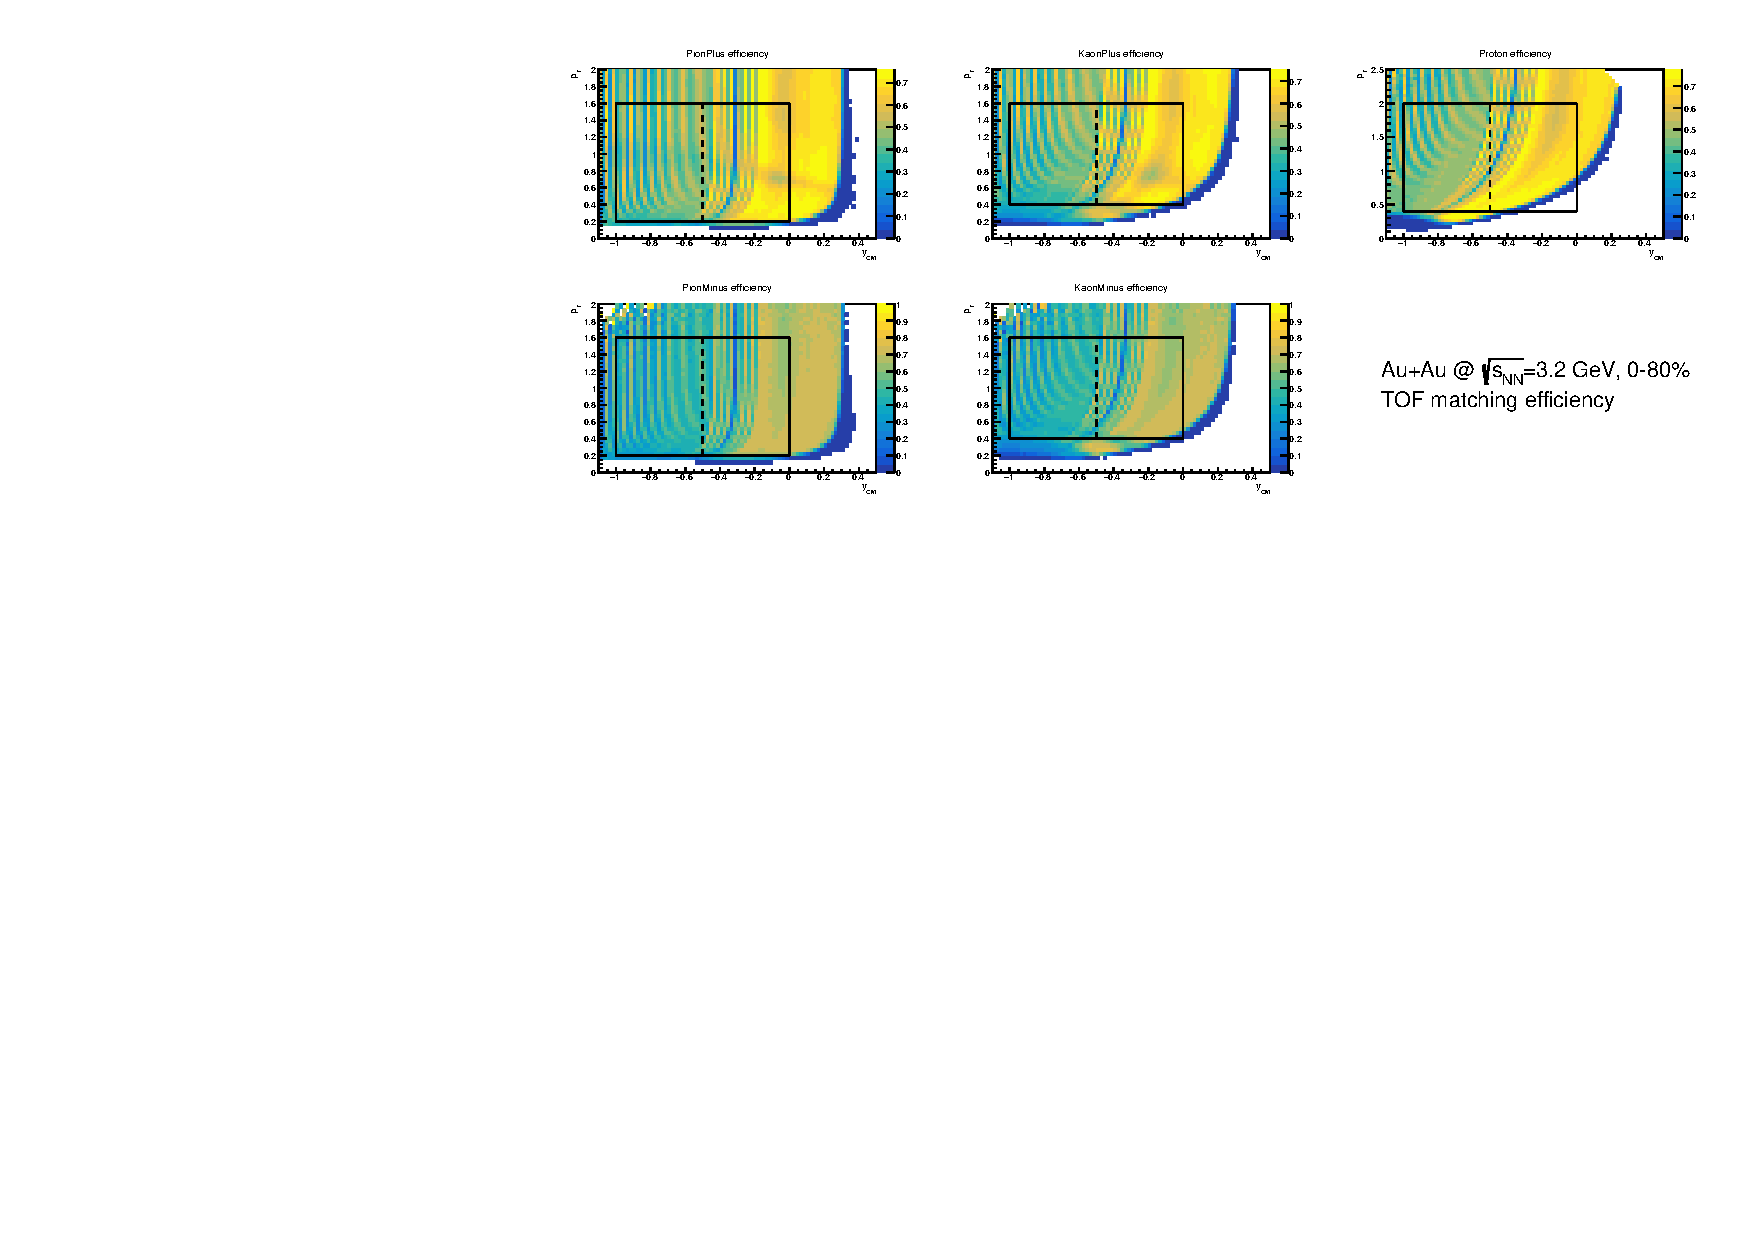
\includegraphics[width=0.65\linewidth]{figures/chapter02/3p2gev_TOF_eff.pdf}
\caption{TOF matching efficiency of $\pi, K, p$ as function of rapidity y and transverse momentum $p_T$ at $\sqrt{s_{NN}}$ = 3.2 GeV.}
\label{fig:3p2_piKp_TOFeff}
\end{figure}

The reconstruction efficiency for $K^{0}_{S}~and~ \Lambda$ can be obtained by the formula~\ref{eq:recon_eff},
which are shown by Fig.~\ref{fig:3p2_K0sLam_eff} at 3.2 GeV. The black box show the measured rapdity and transverse momentum interval, 
where the rapdity cut is $-1<y_{CM}<0$, and $p_T$ cut are $0.2<p_T<1.6, 0.4<p_T<2.0$ for $K^{0}_{S}~and~ \Lambda$, respectively. 
Note that the track and topological cuts applied are identical with identification cuts which is shown by the TABLE.~\ref{tab:K0s_lam_cut}.
For other energies, the TPC tracking efficiency can be found in the appendix.(3GeV(Fig~\ref{fig:3gev_K0sLam_eff}), 3.5GeV, 3.9GeV)
\begin{equation}
    \epsilon\left(p_T, y\right)=\frac{\text {Number of Reconstructed Tracks }}{\text { Number of MC Tracks }}
\label{eq:recon_eff}
\end{equation}

\begin{figure}[hbt!]
\centering
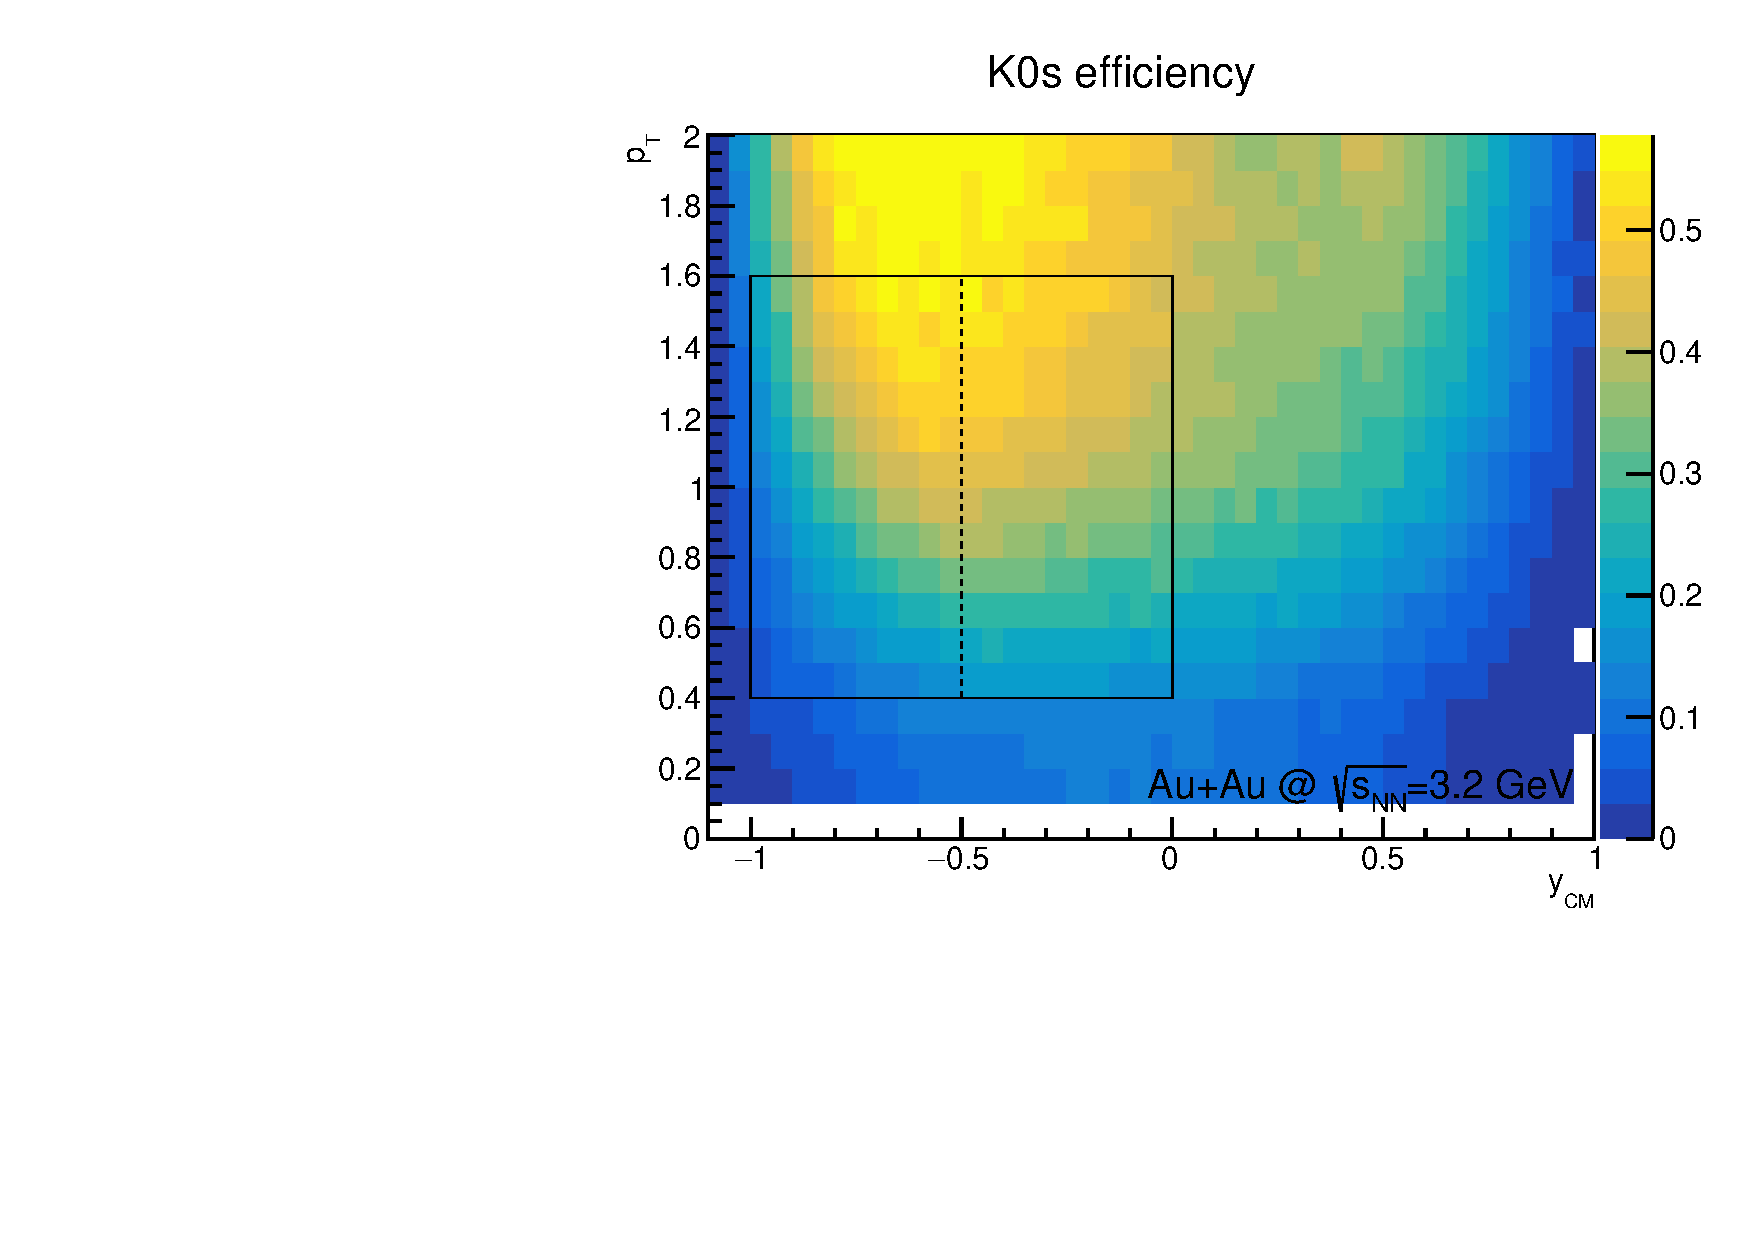
\includegraphics[width=0.45\linewidth]{figures/chapter02/3p2_K0s_eff.pdf}
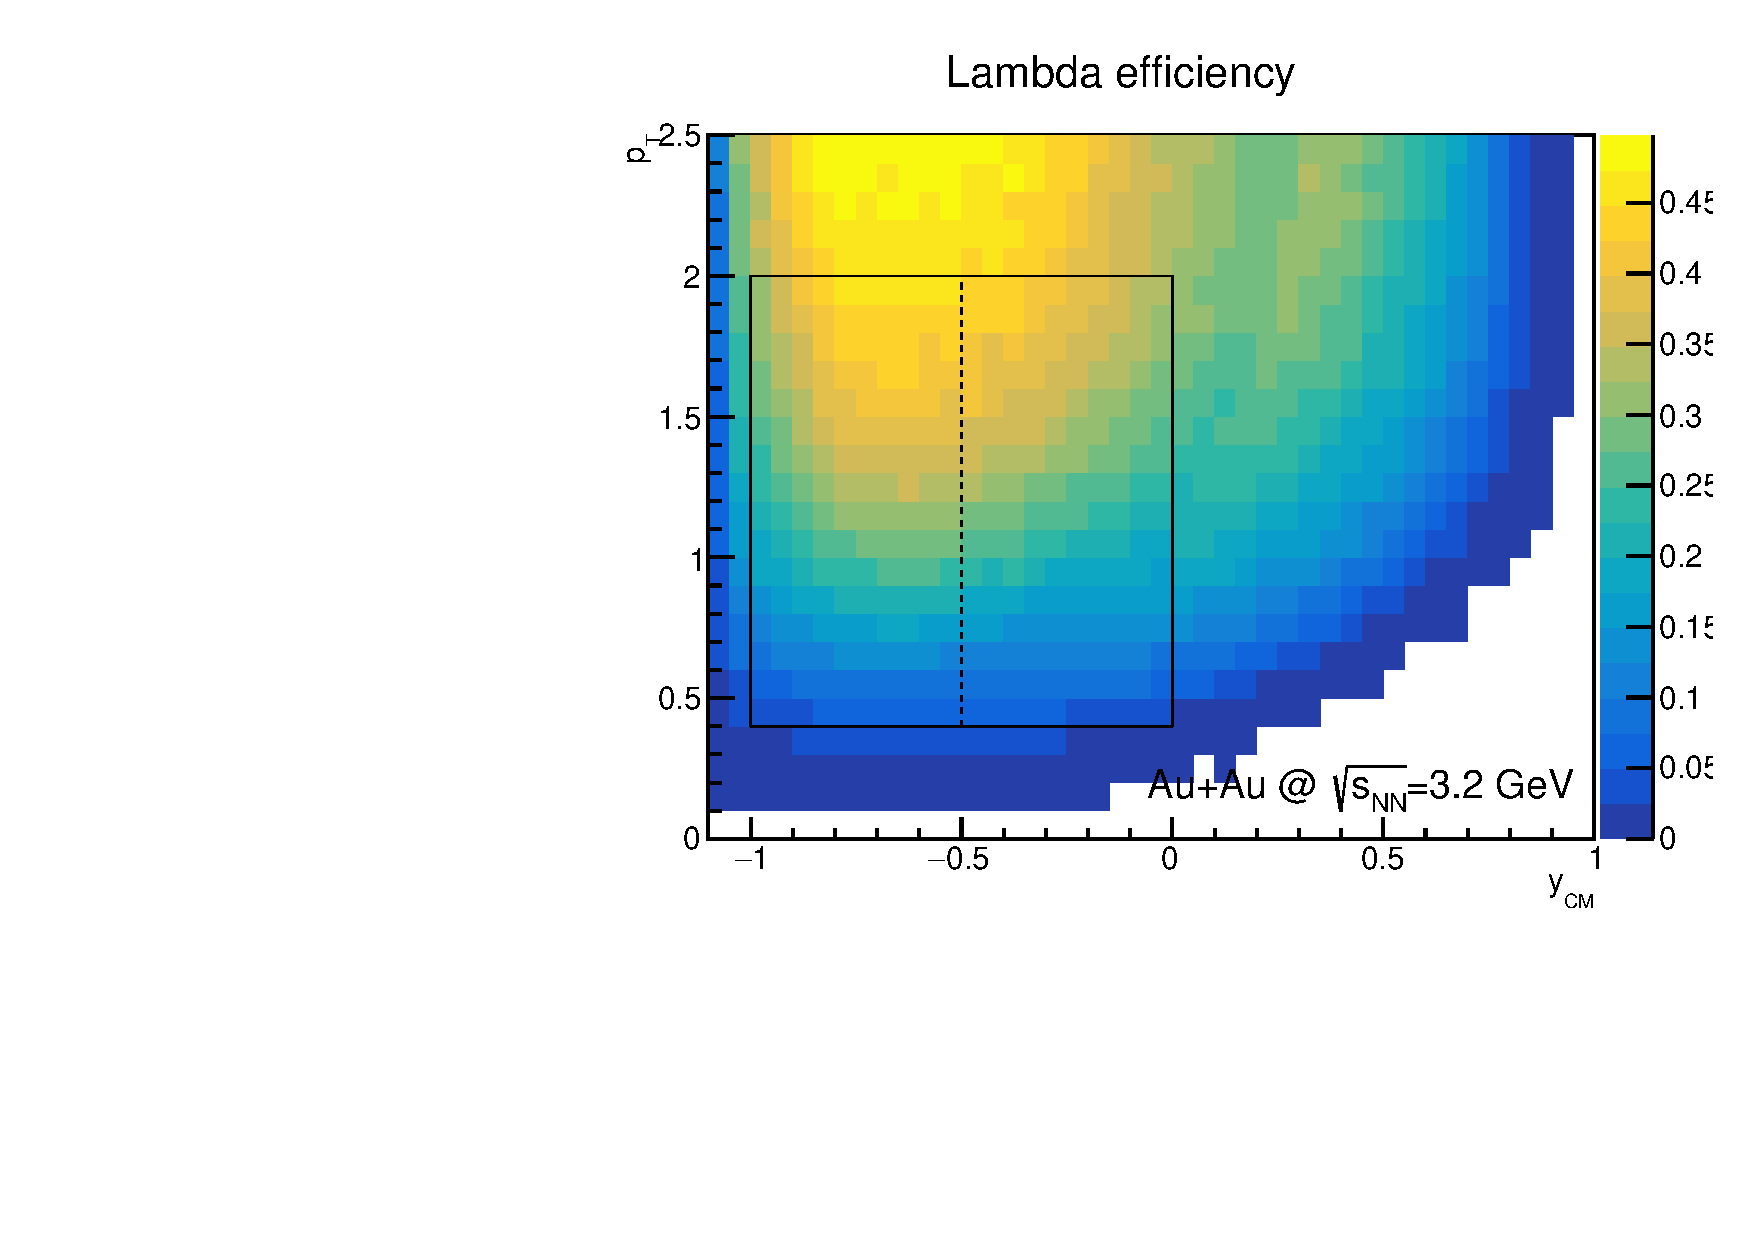
\includegraphics[width=0.45\linewidth]{figures/chapter02/3p2_lambda_eff.pdf}
\caption{Reconstruction efficiency of $K^{0}_{S}(Left), \Lambda(Right)$ as function of rapidity y and transverse momentum $p_T$ at $\sqrt{s_{NN}}$ = 3.2 GeV.}
\label{fig:3p2_K0sLam_eff}
\end{figure}


